\externaldocument{chapter7}
\chapter{Evaluation of ADFD and ADFD$^+$ techniques}
\label{chap:Evaluation}
	
The newly developed ADFD and ADFD$^+$ techniques have been described in detail in the preceding chapters (\ref{chap:ADFD} and~\ref{chap:ADFD+}). Experimental evaluation of the two techniques through purpose built error-seeded numerical programs presented in the two chapters revealed that both techniques were capable of identifying the planted faults effectively. In this chapter, we have evaluated the precision of identifying the failure domains in the two techniques. For this purpose, we have incorporated Daikon in ADFD and ADFD$^+$. Daikon was selected on the basis of its capability to automatically generate invariants of failure domains, precisely point out the boundaries of failure domains and present the failure domains generated in more than two dimensional programs. We have performed extensive experimental analysis of real world Java projects contained in Qualitas Corpus. The results obtained were analysed and cross-checked using manual testing. The impact of nature, location, size, type and complexity of failure domains on the testing techniques were also studied \cite{ahmad2014evaluation}. 




  


%The previous chapters~\ref{chap:ADFD} and~\ref{chap:ADFD+} described the working mechanism of ADFD and ADFD$^+$ techniques along with their experimental evaluation through purpose build error-seeded numerical applications. It was revealed from the experimental results that both the techniques are capable of identifying the planted faults effectively. However to evaluate the effectiveness of the techniques on real-world software applications, we performed an extensive experimental analysis of Java projects contained in Qualitas Corpus. The results obtained were analysed and cross-checked using Manual testing. The impact of nature, location, size, type and complexity of failure domains on the testing techniques were also studied. 

%The results provide insights into the effectiveness of automated techniques and a number of lessons for testing researchers and practitioners.

%\section{abstract}
%The achievement of up-to 50\% better results by Adaptive Random Testing (ART) in comparison with Random Testing (RT) ensures that failure-domains within the input domain are useful and need due consideration in selection of test inputs. Our previously developed two automated techniques (ADFD and ADFD+), automatically find failure and its domain in a specific range and present it graphically.
%They can precisely detect the failure-domain of the identified failure in an effective way. Performing exhaustive testing in a limited region around the failure is the key to the success of ADFD and ADFD+ techniques.

%In this article, we performed an extensive experimental analysis of Java projects contained in Qualitas Corpus for finding the effectiveness of automated techniques (ADFD and ADFD+). The results obtained were analysed and cross-checked using manual testing. The impact of nature, location, size, type and complexity of failure-domains on the testing techniques were studied. The results provide insights into the effectiveness of automated techniques and a number of lessons for testing researchers and practitioners.

%The abstract should summarize the contents of the paper and shouldcontain at least 70 and at most 150 words. It should be written using the \emph{abstract} environment.
%\keywords{We would like to encourage you to list your keywords within the abstract section}





%\section{Introduction}
%The input-domain of a given SUT can be divided into two sub-domains. The pass-domain comprises of the values for which the software behaves correctly and the failure-domain comprises of the values for which the software behaves incorrectly. Chan et al.~\cite{chan1996proportional} observed that input inducing failures are contiguous and form certain geometrical shapes. They divided these into point, block and strip failure-domains as shown in Figure~\ref{fig:patterns}. Adaptive Random Testing achieved up to 50\% better performance than random testing by taking into consideration the presence of failure-domains while selecting the test input~\cite{chen2005adaptive}.

%\smallskip
%\begin{figure} [H]
%\centering
%\subfigure[Point domain]{
%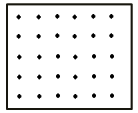
\includegraphics[width=2.5cm,height=2cm]{chapter7/point.png}
%\label{fig:point}
%}
%\subfigure[Block domain]{
%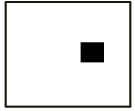
\includegraphics[width=2.5cm,height=2cm]{chapter7/block.png}
%\label{fig:block}
%}
%\subfigure[Strip domain]{
%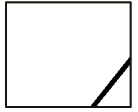
\includegraphics[width=2.5cm,height=2cm]{chapter7/strip.png}
%\label{fig:strip}
%}
%\smallskip
%\caption{Failure domains across input domain~\cite{chan1996proportional}}
%\label{fig:patterns}
%\end{figure} 

%Adaptive Random Testing (ART) exploited the existence of the failure-domains and resultantly achieved up to 50\% better performance than random testing~\cite{Chen2008}. This was mainly attributed to the better distribution of input which increased the chance of selecting inputs from failure-domains. This insight motivated us to increase our understanding of failure-domains in production software.

%The cost of software testing constitute about half of the total cost of software development~\cite{myers2011art}. Software testing is an expensive but essential process which is particularly time consuming, laborious and error-prone when performed manually. Alternatively, automated software testing may involve higher initial cost but brings the key benefits of lower cost of production, higher productivity, maximum availability, greater reliability, better performance and ultimately proves highly beneficial for any organisation~\cite{beizer2003software}. A case study conducted by Pacheco et al. reveals that the 150 hours of automated testing found more faults in complex .NET code than a test engineer finds in one year by manual testing~\cite{pacheco2008finding}.

%We have developed two fully automated techniques ADFD~\cite{ahmad2013adfd} and ADFD+~\cite{ahmad2014adfd2}, which effectively find failures and their domains in a specified range and also provide visualisation of the pass and fail domains. The process is accomplished in two steps. In the first step, an upgraded random testing is used to find the failure. In the second step, exhaustive testing is performed in a limited region around the detected failure in order to identify the domains. The ADFD searches in one-dimension and covers longer range than ADFD+ which is more effective in multi-dimension and covers shorter range.

%Three separate tools including YETI, Daikon and JFreeChart have been used in combination to develop ADFD and ADFD+ techniques. The York Extensible Testing Infrastructure~\cite{Oriol2011yeti} is used to test the program automatically with ADFD or ADFD+ strategy. The Daikon~\cite{ernst2007daikon} checks all test executions and automatically generates invariants to present failure-domains quantitatively. The JFreeChart~\cite{gilbert2008jfreechart} facilitates graphical representation of the pass and fail domains.

%Software testing can be performed either automatically or manually. Both the techniques have their own advantages and limitations. The main advantage of automated testing is execution of large number of tests in little time, whereas manual testing utilizes the tester experience to concentrate on error-prone part of the SUT and generate target oriented test cases~\cite{Leitner2007}. 

%The analysis of failures and failure-domains discovered in 57 classes from 25 open source Java projects of Qualitas Corpus through three different techniques---ADFD, ADFD+ and Manual testing---reveals that each is good at uncovering different type of failure-domains and each brings distinct contributions.


%The rest of the paper is organized as follows: Section 2 presents enhancement of the techniques. Section 3 shows the difference in working mechanism of the two techniques by a motivating example. Section 4 highlights the key research questions. Section 5 explains the evaluation process, which contain experiments, results and answers of research questions in view of experiment results. Section 6 presents the threats to validity. Section 7 presents related work. Finally, Section 8 concludes the study.


 

%%%%%%%%%%%%%%%%%    ADFD and ADFD+   %%%%%%%%%%%%%%%%%%%

%\section{Automated Techniques}
%The two automated techniques used in our experiments are ADFD and ADFD+. A short overview of both the techniques and the enhancements that have been made to the techniques along with a motivating example are given below:

%\subsection{Overview of ADFD technique}
%Automated Discovery of Failure Domain is an automated technique for finding and drawing the failure domain of detected failure in the input domain. ADFD searches for failure domain between the specified lower and upper bound in uni-direction. It test and note only the ranges of pass and fail values and uses the scatter graph of the JFreeChart to plot them on the screen. For more details please see \cite{ahmad2013adfd}.

%\subsection{Overview of ADFD+ technique}
%Automated Discovery of Failure Domain+ is an automated technique for finding and drawing the failure domain of detected failure in the input domain. ADFD+ searches for failure domain around the failure in specified range in multi-idirection. It test and note individual value as either pass or fail. The values are drawn using the vector graph of the JFreeChart. For more details please see \cite{ahmad2014adfd2}.



\section{Enhancement of the Techniques}
Prior to experimental evaluation, new features were incorporated in ADFD and ADFD$^+$ techniques to: increase the code coverage, provide information about the identified failure and generate invariants of the detected failure domains as stated below: 
\begin{enumerate}

\item The GUI is enabled to launch all the strategies defined in YETI from a single interface. For example: if ADFD strategy is selected for testing the system automatically hides the field associated with ADFD+ (range value) and displays two fields of lower and upper bounds. On the other hand if ADFD$^+$ strategy is selected for testing, the system automatically hides the two fields associated with ADFD technique (lower and upper bounds) and displays a single field of range value.

\clearpage
\newpage 

\item Code coverage was increased by extending the techniques to support the testing of methods with \verb+byte, short, long, double+ and \verb+float+ type arguments while it was restricted to \verb+int+ type arguments only in the original techniques.

\item Invariants of the detected failure domains were automatically generated by integrating the tool Daikon in the two techniques. Daikon is an automated invariant detector that detects likely invariants in the program~\cite{ernst2007daikon}. The generated invariants are displayed in GUI at the end of test execution. 

\item Additional information was facilitated by adding the YETI generated failure finding test case to the GUI of the two techniques. Test case included type of failure, name of the failing class, name of the failing method, values causing the failure and line number of the code causing failure.


%\begin{figure}
%\centering
% \makebox[\textwidth][c]{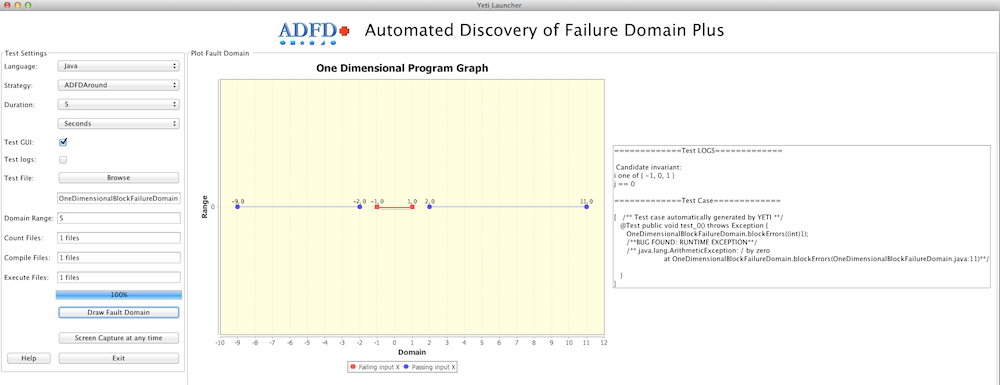
\includegraphics[width=1.25\textwidth, height=10cm]{chapter7/adfdUpgraded1.png}}%
% \bigskip
%  \caption{GUI front end of upgraded ADFD and ADFD$^+$}
%  \label{fig:adfdUpgraded}
%\end{figure}
%\bigskip
%\bigskip


%\begin{figure}[ht]

%\centering
%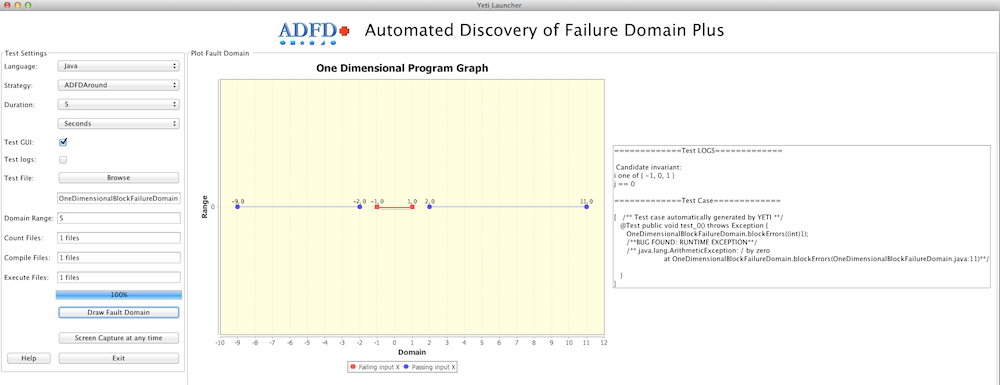
\includegraphics[width= 17.5cm,height=11cm]{chapter7/adfdUpgraded1.png}
%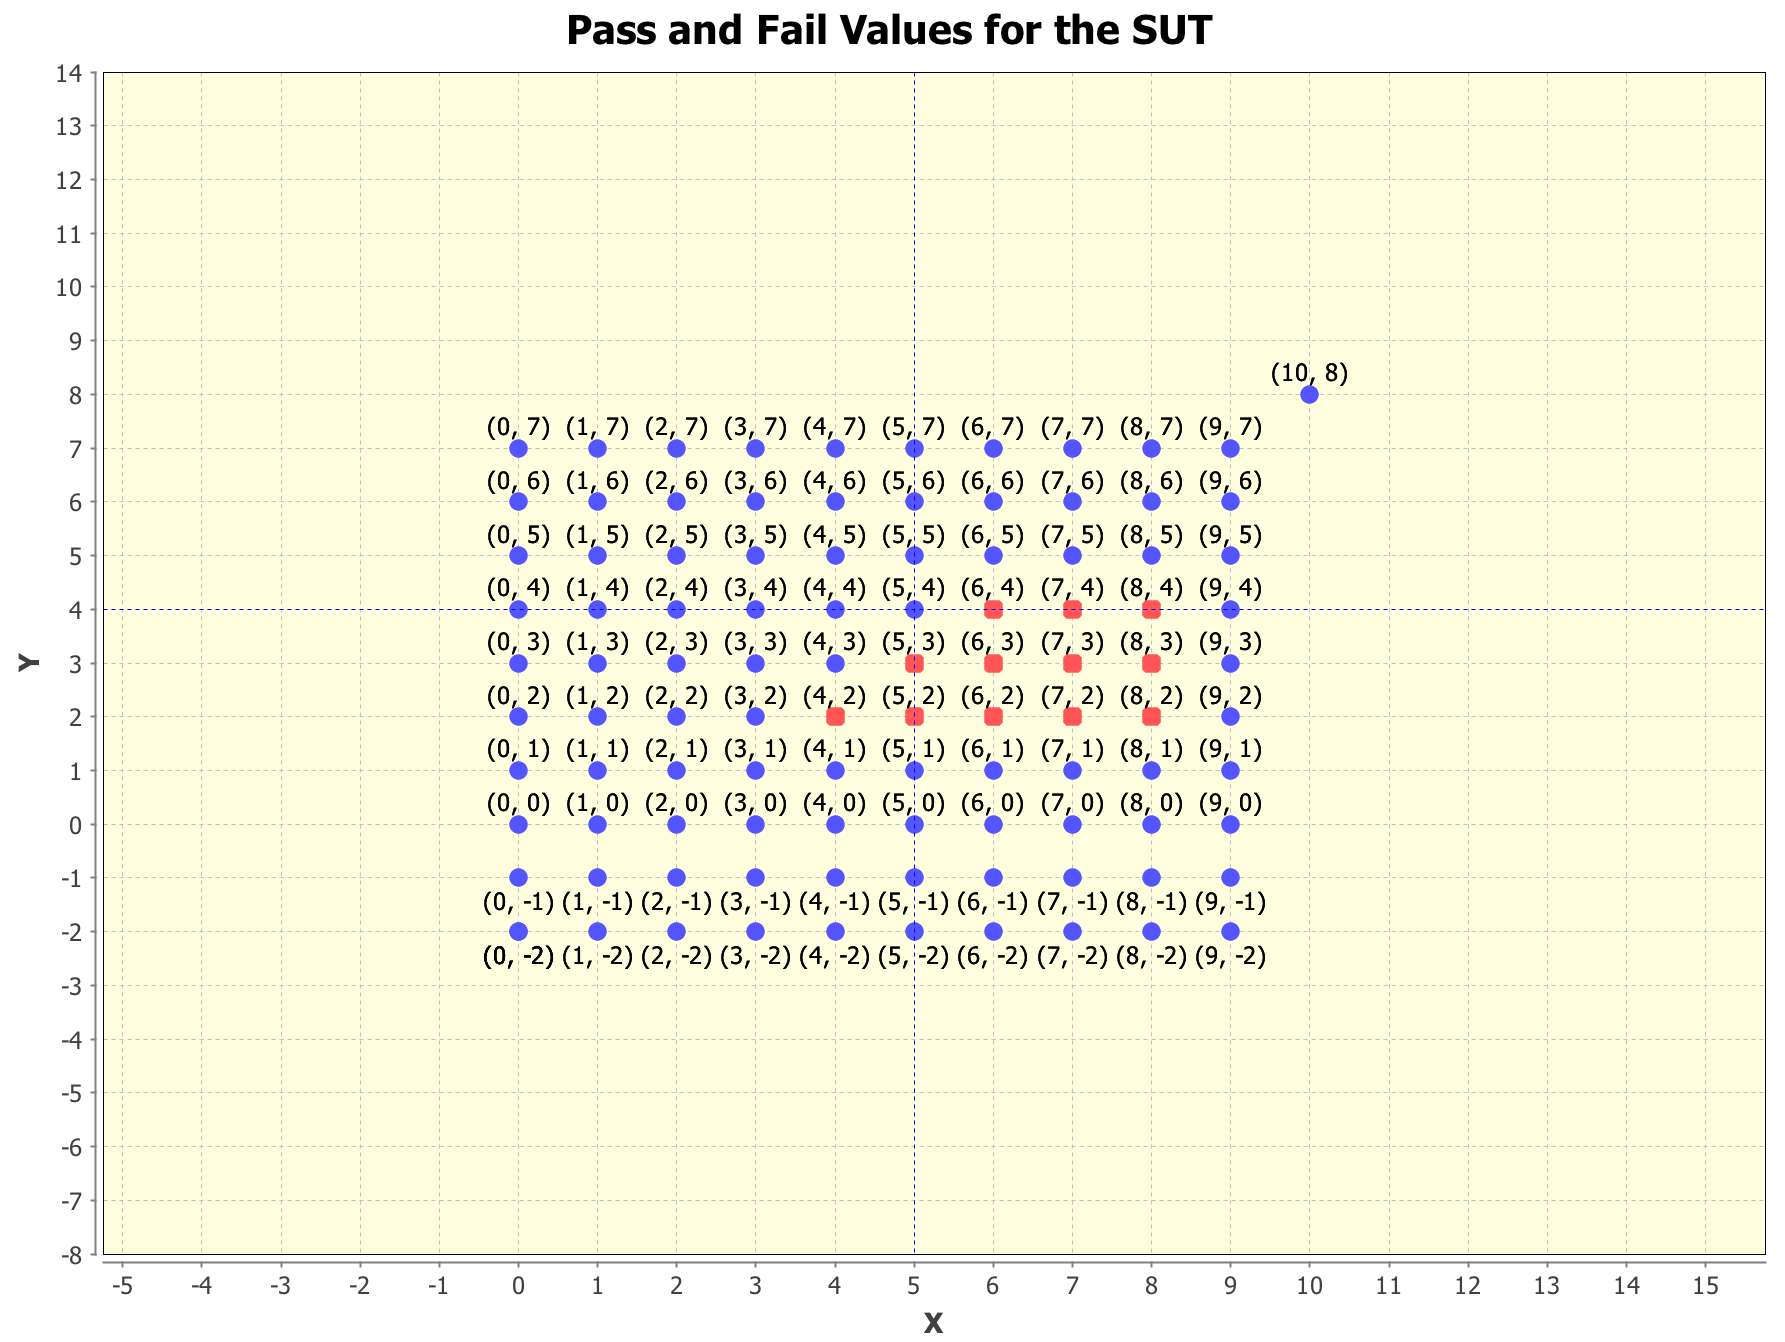
\includegraphics[width= 8.5cm,height=7cm]{adfdPlus1.png}
%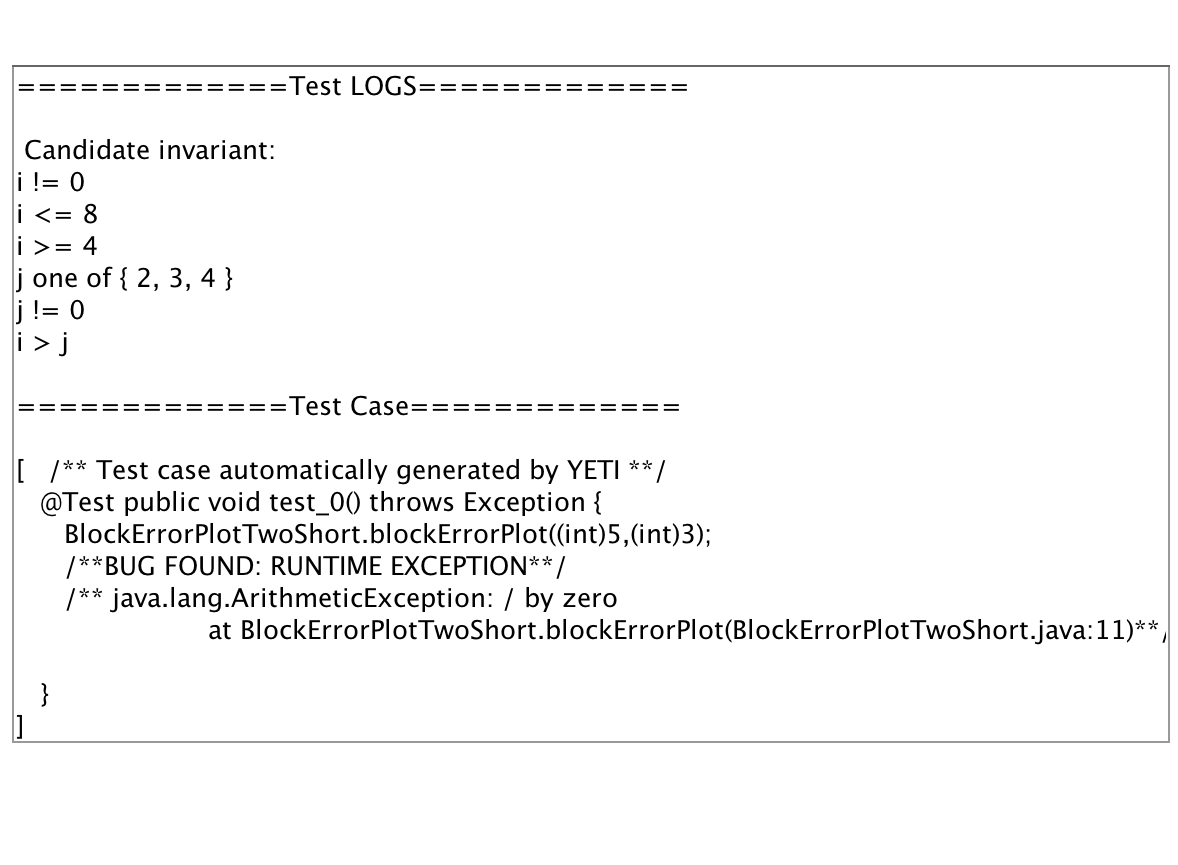
\includegraphics[width= 8.5cm,height=7cm]{adfdPlus2.png}
%\bigskip
%\caption{GUI front end of upgraded ADFD and ADFD$^+$}
%\label{fig:adfdUpgraded}
%\end{figure}

\item The feature of screen capture is added to the new GUI. User can click the screen capture button to capture the current screen during the testing process. It allows the user to capture multiple screen-shots at different intervals of testing for future reference. 

\end{enumerate}
\bigskip



Four of the above enhancements are visible from the front-end. As shown in Figure~\ref{fig:adfdUpgraded}, the drop down menu for strategy field enables the tester to choose the appropriate strategy in the list for the test session. Secondly, the block failure domain is shown in graphical form and with the help of automatic tool Daikon the failure domain is also shown  by invariants ( i one of \{-1, 0, 1\}, j == 0). Thirdly, the addition of YETI generated test case shows type of failure (RUNTIME EXCEPTION, java.lang.ArithmaticException: / by zero), name of the failing class (OneDimensionalBlockFailureDomain), name of the failing method (blockErrors), value causing the failure (1) and line number of the code causing failure (11). Fourthly, the provision of screen capture button allows the tester to store the record of each test for record.
\clearpage
\newpage


\begin{sidewaysfigure}[ht]
\centering
\centerline{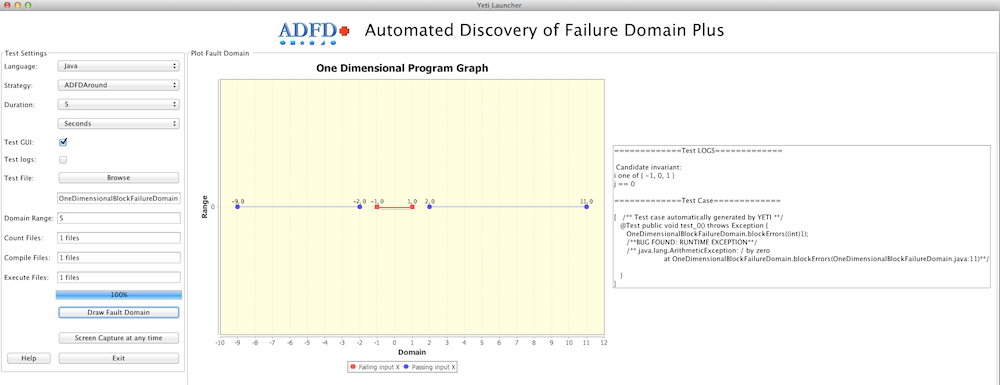
\includegraphics[width=22cm,height=14cm]{chapter7/adfdUpgraded1.png}}
%\centerline{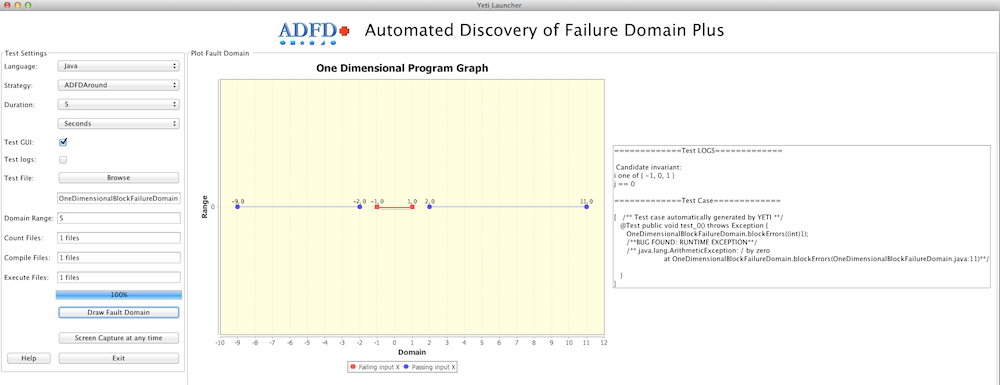
\includegraphics[width=12cm,height=10cm]{chapter7/adfdUpgraded1.png}}
%\includegraphics[width=14cm,height=20cm]{myfigures/plan/project_table.pdf}
\caption{GUI front end of upgraded ADFD and ADFD$^+$}
\label{fig:adfdUpgraded}
\end{sidewaysfigure}


%Three out of five enhancement in the technique are visible from the front-end as shown in Figure~\ref{fig:adfdUpgraded}. It shows the block failure domain with the help of graph and invariants. It further shows that the failure domain is caused by individual failures i.e. when the value of the argument to the method is -1, 0 or 1. The test case generated by YETI shows the type of failure, the first value that caused the failure (1 in this case) and the stack trace of the failure. Finally, the screen capture button is there to capture the screen at any time during the test. The screen capture feature is used to store the record of each test for record.

\clearpage
\newpage
\section{Daikon}
Daikon is an automated tool that detects likely invariants at specific points in the program from execution trace file~\cite{ernst2007daikon}. The trace file records effect of inputs to the program under observation during execution of the test cases. Daikon is capable of generating invariants for programs written in Java, C, C++, Perl and Eiffel. The tool helps programmers by identifying program properties, which must be preserved during modification of the program code. Daikon's output can also provide assistance on understanding, modifying and testing of programs that contain no explicit invariants.

Figure~\ref{fig:daikon} presents the architecture of Daikon. To generate invariants for the original program, Daikon instruments the source code by inserting checks at various points in the program. The checks inserted do not change the original behaviour of the program in any way. On executing the instrumented program the check points collect values of variables accessible to the point and store them in the trace file. The Daikon's inference engine analyse the trace file for any pattern which is true in all samples and reports it as invariant. In order to avoid reporting of any false positive invariant, confidence of each invariant is calculated by Daikon and only that invariant is reported which qualify the set level of confidence. 

\bigskip
\begin{figure}[H]
\centering
%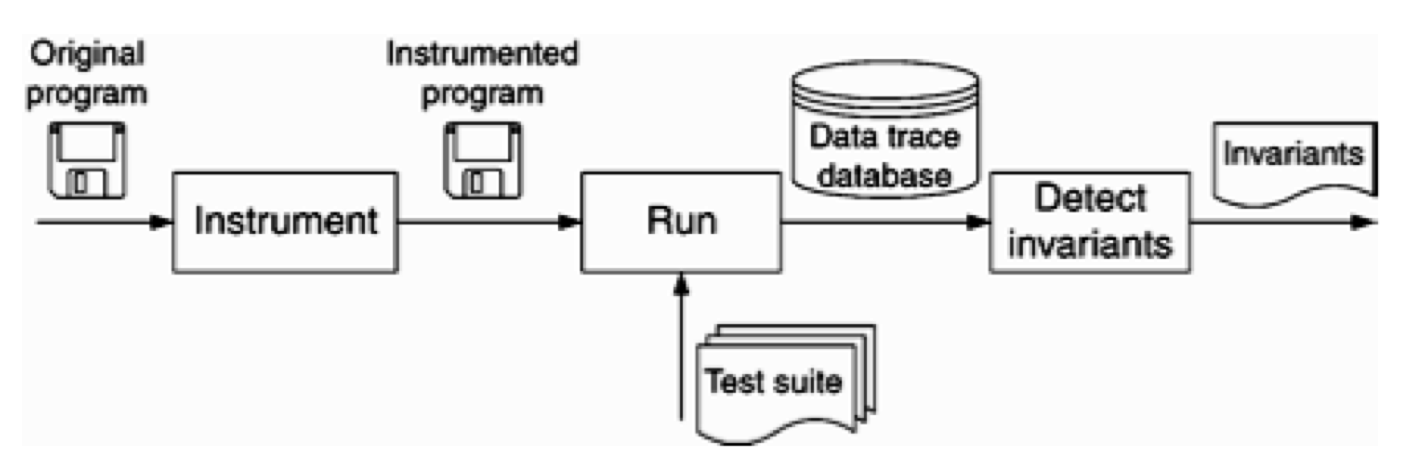
\includegraphics[width= 15.5cm,height=5.5cm]{chapter7/daikon.png}
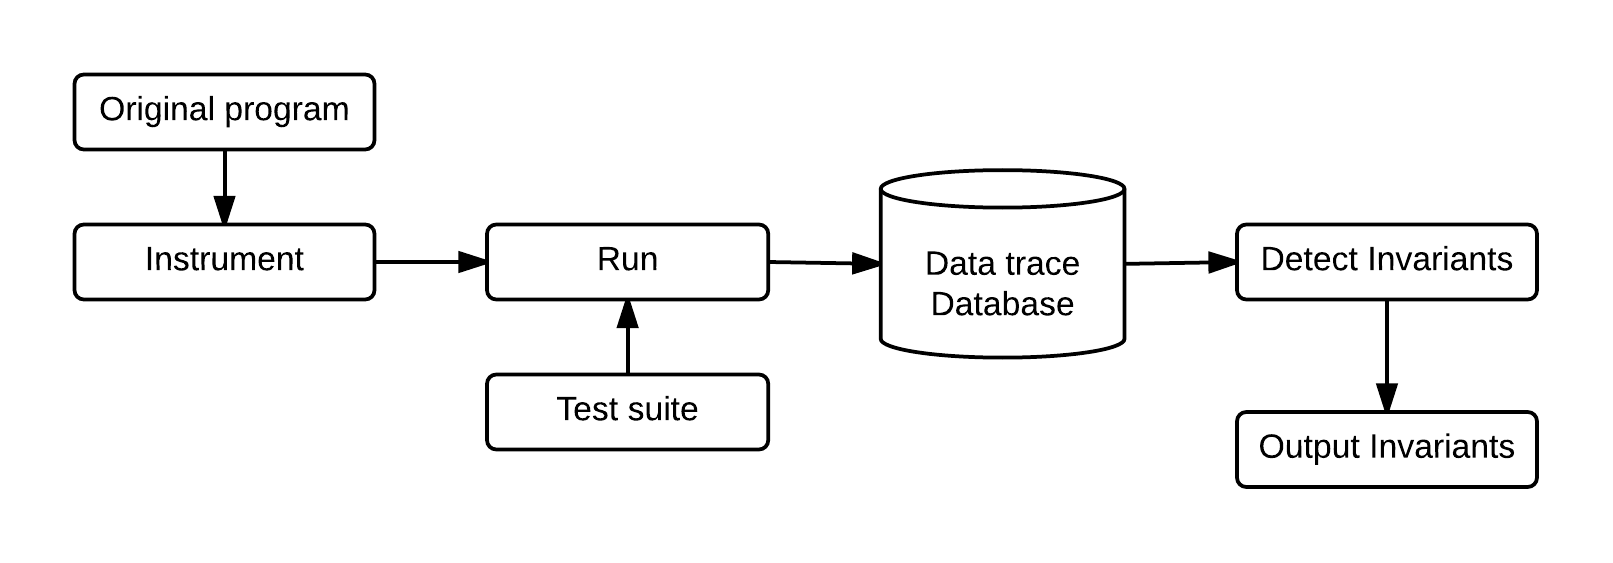
\includegraphics[width= 15.5cm,height=5.5cm]{chapter7/daikonWorking1.png}
\bigskip
\caption{Architecture of Daikon~\cite{ernst2001dynamically}}
\label{fig:daikon}
\end{figure}
\bigskip

\subsection{Types of Invariants Detected by Daikon}
Daikon is usually used to detect common types of likely invariants. However, it can be used to search for more specific invariants if it is tuned for the purpose by the user. The most common types of invariants detected by Daikon are quoted below ~\cite{ernst2001dynamically}. 
\begin{enumerate}
\item Invariants over any variable: 
	\begin{enumerate}
	 \item Constant value: x = a indicates the variable is a constant.
	 \item Uninitialized: x = uninit indicates the variable is never set.
	 \item Small value set: x $\in$ \{a,b,c\} indicates the variable takes only a small number of different values.
	\end{enumerate}
\item Invariants over a single numeric variable: 
	\begin{enumerate}
	\item Range limits: x $\ge$ a; x $\le$ b; and a $\le$ x $\le$ b (printed as x in [a..b]) indicate the minimum and/or maximum value.
	\item Nonzero: x $\ne$ 0 indicates the variable is never set to 0. 
	\item Modulus: x $\equiv$ a mod b indicates that x mod b $\equiv$ a always holds.
	\item Nonmodulus: x $\ne$ a mod b is reported only if x mod b takes on every value beside a.
	\end{enumerate}
\item Invariants over two numeric variables: 
	\begin{enumerate}
	\item Linear relationship: y = ax + b. 
	\item Ordering comparison. 
	\item Invariants over x + y: any invariant from the list of invariants over a single numeric variable.
	\item Invariants over x - y: as for x + y
	\end{enumerate}
\item Invariants over a single sequence variable (arrays): 
	\begin{enumerate}
	\item Range: minimum and maximum sequence values, ordered lexicographically. 
	\item Element ordering: whether the elements of each sequence are non-decreasing, non-increasing or equal.
	\item Invariants over all sequence elements (treated as a single large collection): for example, all elements of an array are at least 100.
	\end{enumerate}
\item Invariants over two sequence variables: 
	\begin{enumerate}
	\item Linear relationship: y = ax + b, elementwise. 
	\item Comparison: lexicographic comparison of elements. 
	\item Subsequence relationship.
	\end{enumerate}
\end{enumerate}

% check generating high confident invariants thesis for it.







\section{Difference in Working Mechanism of the Two Techniques}
Difference in working mechanism of ADFD and ADFD$^+$ for identification of failure domains is illustrated by testing a simple Java program (given below) with the two techniques. 
\bigskip
\begin{lstlisting}
/** 
* A program with block failure domain.
* @author (Mian and Manuel)
*/
public class BlockErrorPlotTwoShort {
	public static void blockErrorPlot (int x, int y) {
		if ((x >= 4) && (x <= 8) && (y == 2)) { 
			abort();		/* error */
		}
		if ((x >= 5) && (x <= 8) && (y == 3)) { 
			abort();		/* error */
		}
		if ((x >= 6) && (x <= 8) && (y == 4)) { 
			abort();		/* error */
		}
	}
}
\end{lstlisting}
\bigskip


As evident from the program code, a failure is generated when the value of variable \textit{x = \{4, 5, 6, 7 or 8\}} and the corresponding value of variable \textit{y = \{2, 3 or 4\}}. The total number of 12 failing instances form a block failure domain in the input domain.

The test output generated by ADFD technique is presented in Figure~\ref{fig:ADFD}. The labelled graph shows only 4 out of 12 failing values in red whereas the passing values are shown in blue. The generated invariants identify all but one failing value ($x = 4$). This is due to the fact that ADFD scans the values in one-dimension around the failure. The test case shows the type of failure, name of the failing class, name of the failing method, values causing the failure and line number of the code causing failure.

The test output generated by ADFD$^+$ technique is presented in Figure~\ref{fig:ADFD+}. The labelled graph correctly shows all the 12 out of 12 available failing values in red whereas the passing values are shown in blue. The invariants correctly represent the failure domain. The test case shows the type of failure, name of the failing class, name of the failing method, values causing the failure and line number of the code causing failure.



\begin{figure}[H]
\centering
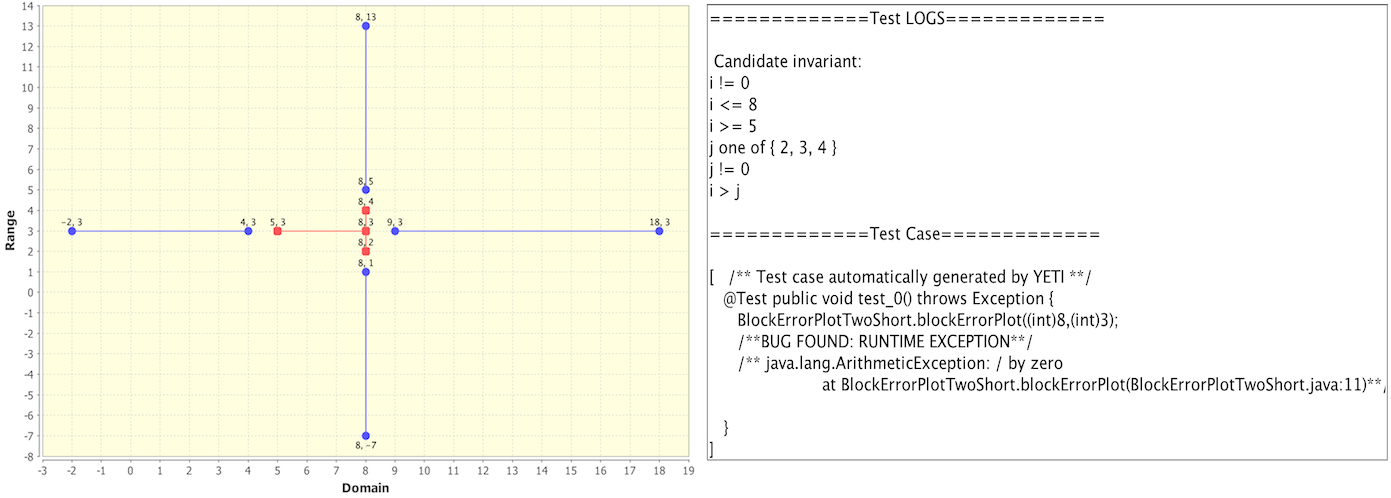
\includegraphics[width= 15.5cm,height=8cm]{chapter7/adfdCombined.png}
%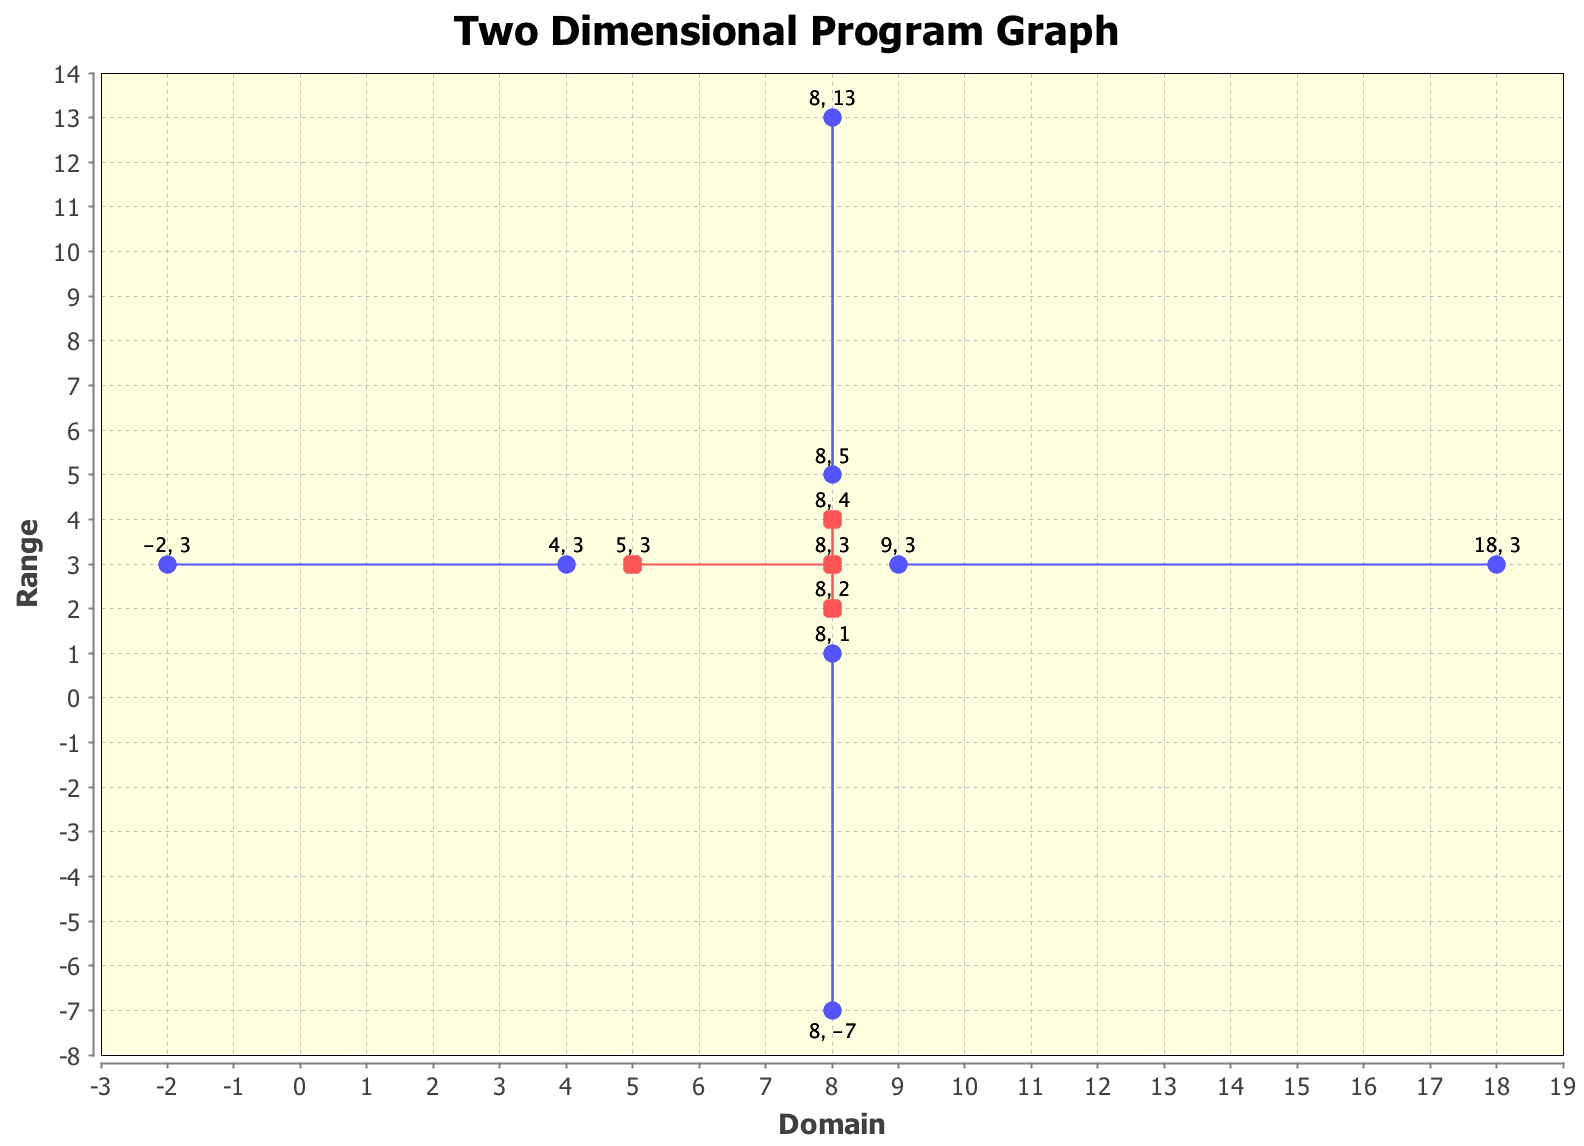
\includegraphics[width= 8.5cm,height=7cm]{adfdAround1.png}
%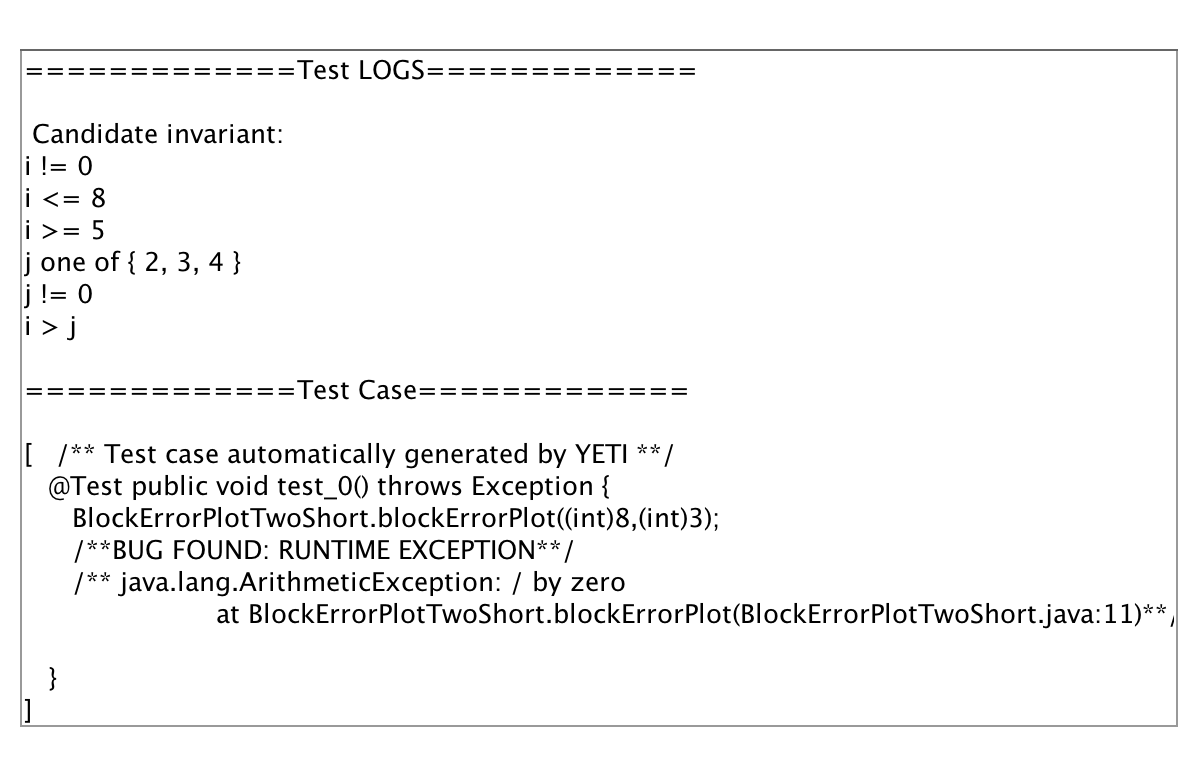
\includegraphics[width= 8.5cm,height=7cm]{adfdAround2.png}
\caption{Graph, Invariants and test case generated by ADFD for the given code}
\label{fig:ADFD}
\end{figure}


\bigskip
\bigskip
\begin{figure}[H]
\centering
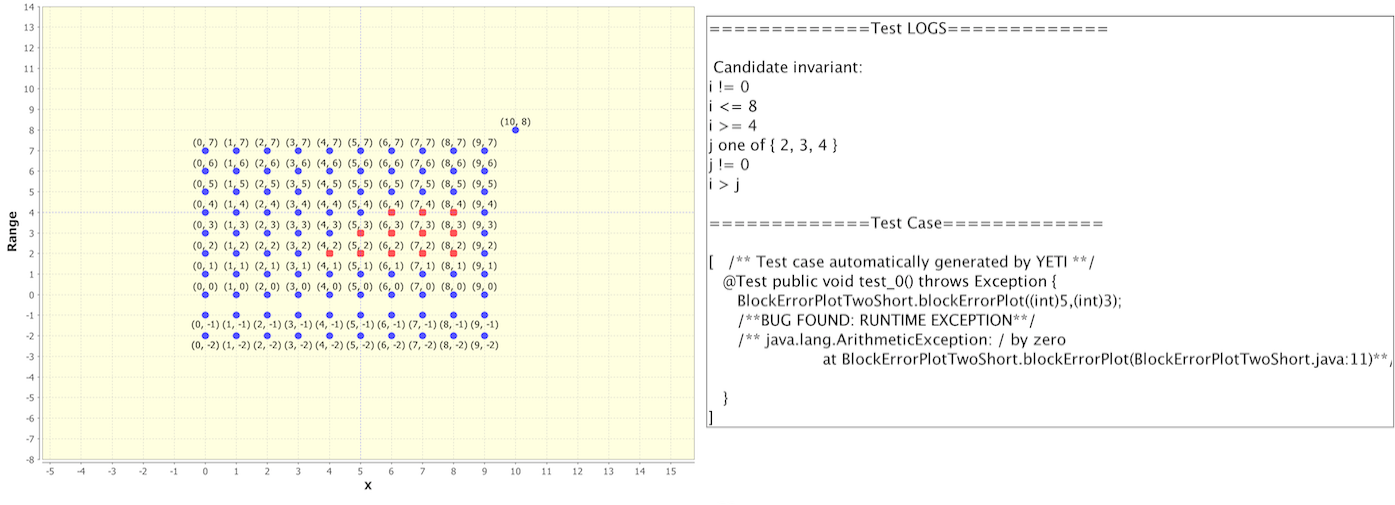
\includegraphics[width= 15.5cm,height=8cm]{chapter7/adfdPlusCombined.png}
%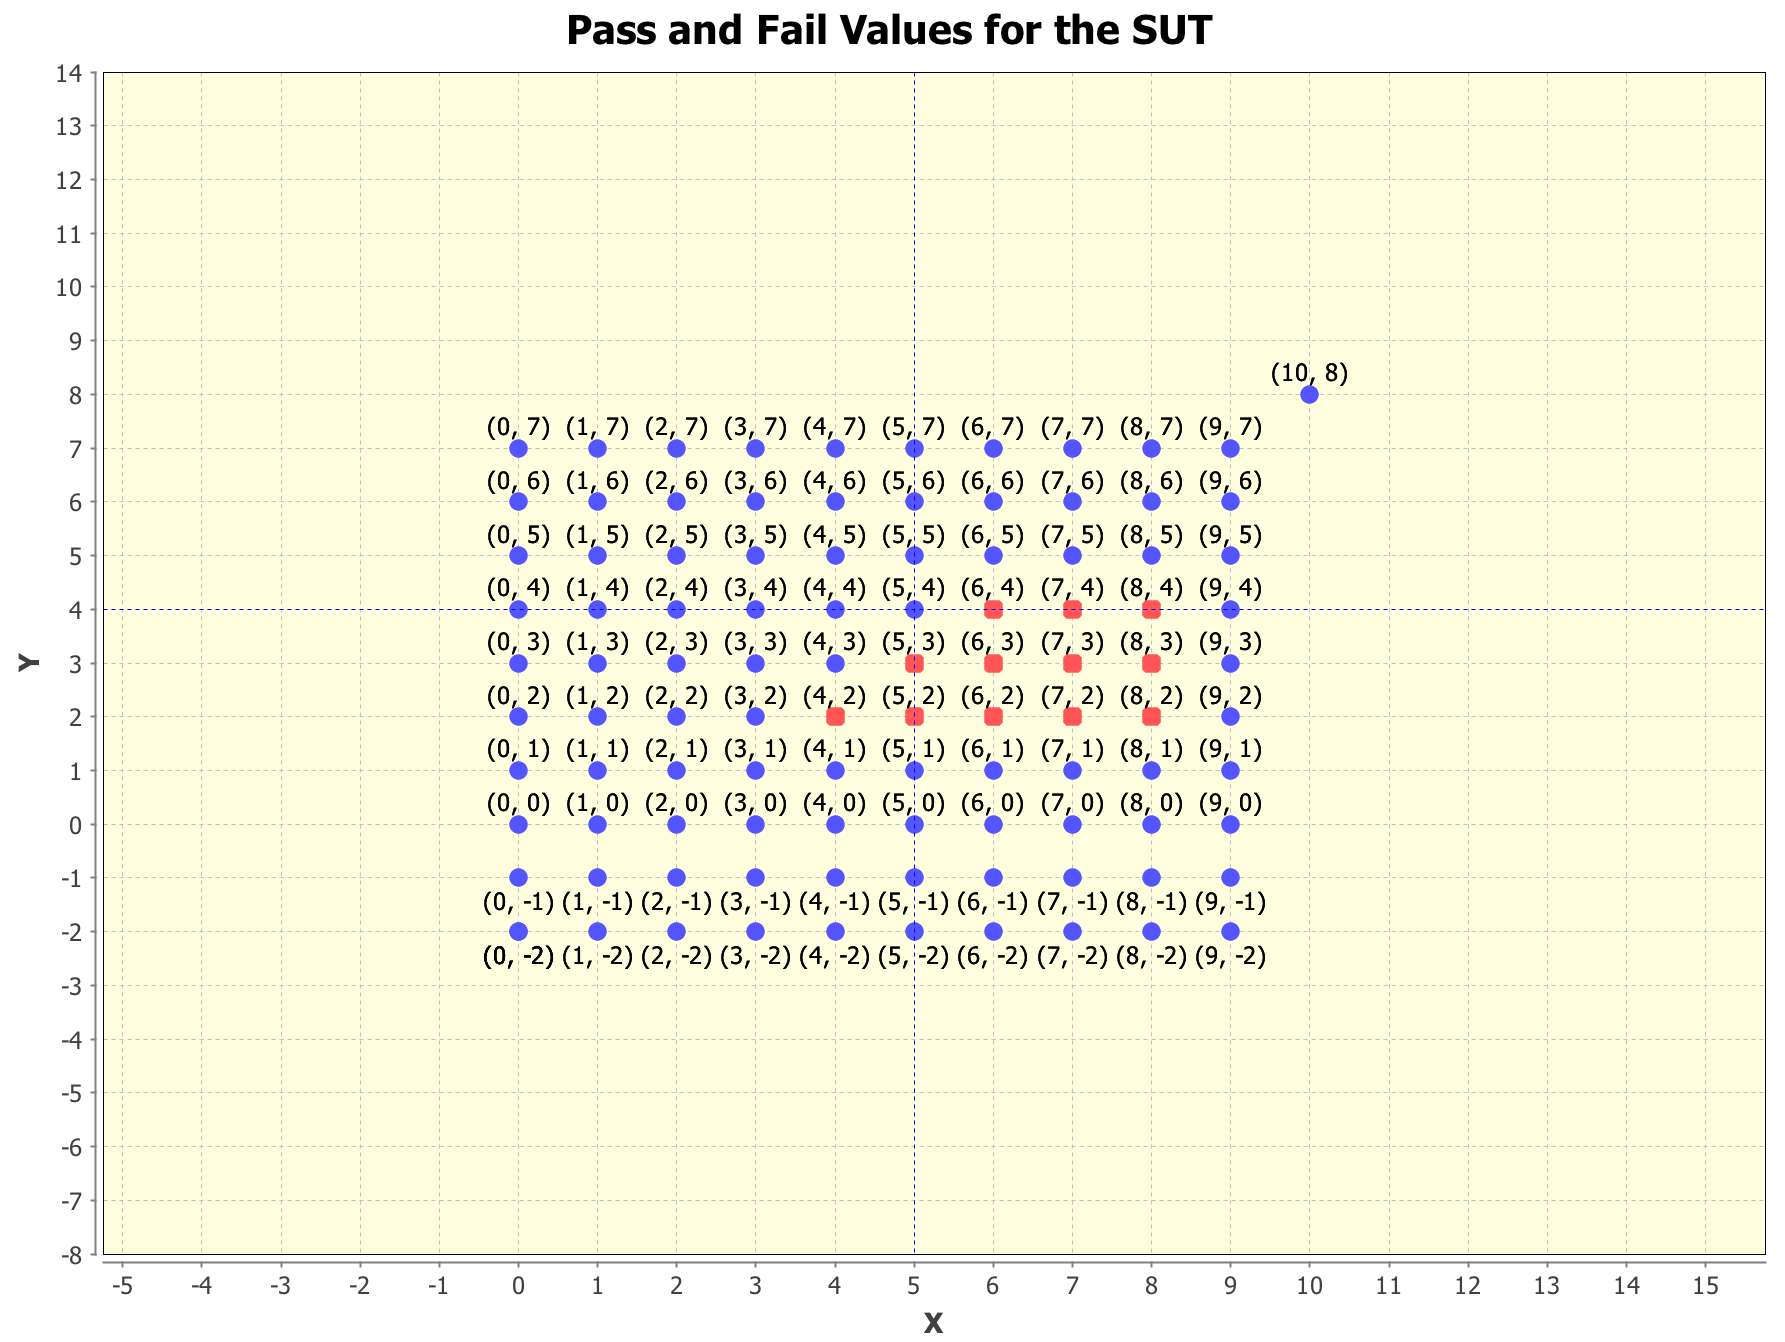
\includegraphics[width= 8.5cm,height=7cm]{adfdPlus1.png}
%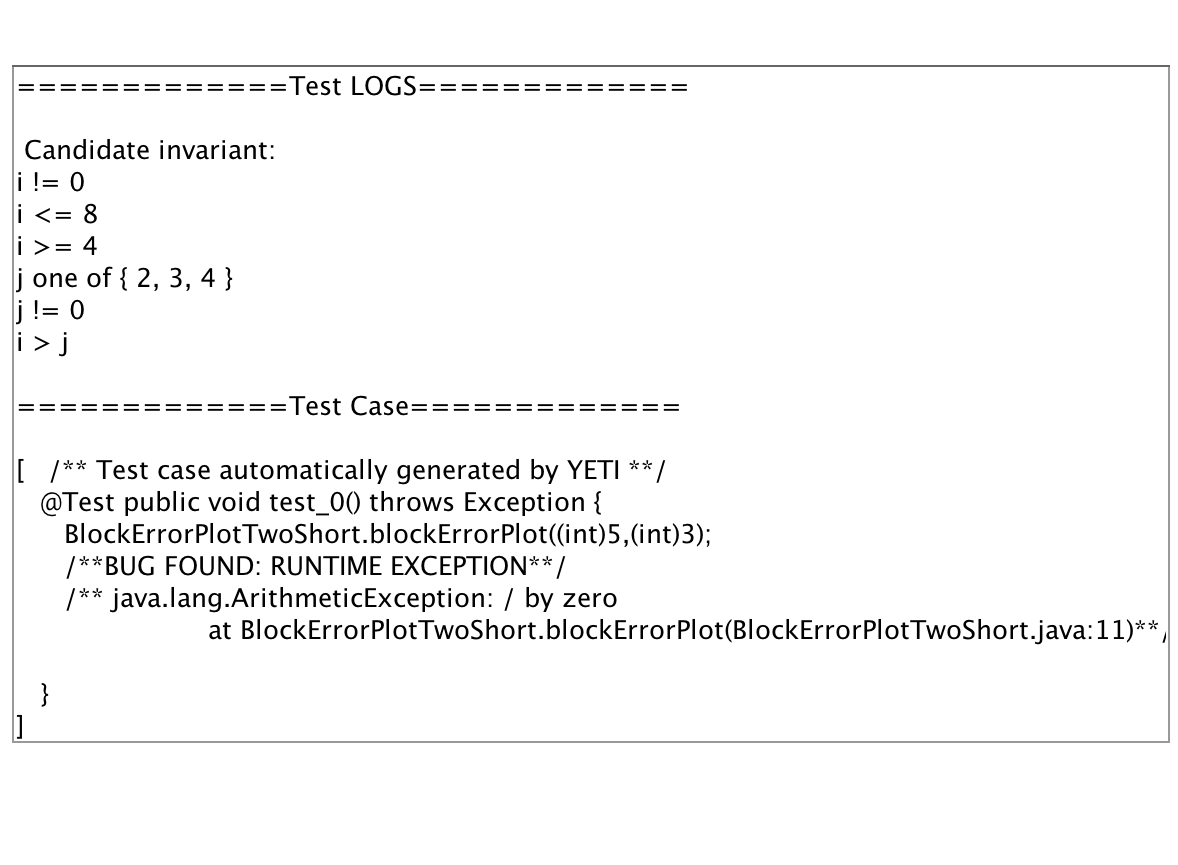
\includegraphics[width= 8.5cm,height=7cm]{adfdPlus2.png}
\caption{Graph, Invariants and Test case generated by ADFD$^+$ for the given code}
\label{fig:ADFD+}
\end{figure}
\bigskip



The comparative results derived from execution of the two techniques on the developed program indicate that, ADFD$^+$ is more efficient than ADFD in identification of failures in two-dimensional programs. The ADFD and ADFD$^+$ performs equally well in one-dimensional program, but ADFD covers more range around the first failure than ADFD$^+$ and is comparatively economical because it uses fewer resources than ADFD$^+$.


\section{Research Questions} \label{sec:questions}
The following research questions have been addressed in the study:
\begin{enumerate}
%
\item What is the relevance of ADFD and ADFD$^+$ techniques in identification and presentation of failure domains in production software? %\\%The experimental results claiming the correct identification of ADFD and ADFD+ were based on the purpose build error-seeded programs~\cite{}. To answer the question, we applied the two techniques to all the projects of Qualitas Corpus and examined the results.

%\item \textit{If the graph and invariants generated, correctly represent the failure domains?} %Invariants generated by Daikon can identify the start and stop of the failure domain. To answer this question we compared the generated invariants with the source code and the failure-domain presented in graphical form.
%
%
\item What types and frequencies of failure domains exist in production software? %\\%There are strategies~\cite{}.  that exploit the presence of block and strip failure-domain to get better results. Therefore identifying the presence of underlying failure-domains in production software can help in high quality of software testing.  To answer the questions, we reviewed all the classes containing failure-domains manually, automatically and graphically.
%
\item What is the nature of identified failure domain and how it affects the automated testing techniques? % \\% An interesting point is to know what failure is responsible for a failure-domain and how difficult it is to identify that failure by manual testing. To answer this question, we studied the test logs and test output of the automated testing and the source code of the program manually to identify the cause and complexity of failures of failure-domains. 

%\item \textit{If the presence of a particular failure-domain can make it easy or hard to find using automated and manual techniques?} 
%Failure-domain can reside in the form of point, block or strip shape in the input domain. To answer this question we analysed the source code of all the programs in which failure-domains were detected.
%

%\item \textit{If the graph generated by ADFD correctly represent the pass and fail domains?} Both the ADFD and ADFD+ techniques generate graphs to represent failure-domains for simplicity. To answer the question we compared the generated graphs with the source code and the invariants generated by Daikon.
%
%\item If obtained results consistent with previous theoretical and practical results presented?  %As per our knowledge, till now no specific study has been conducted to automatically identify the pass and fail domains however it has been claimed by some researchers~\cite{} that there exist more block and strip patterns then the point patterns. 
%

%\item What is the external validity of the results obtained?\\

\end{enumerate}




\section{Evaluation}
Experimental evaluation of ADFD and ADFD$^+$ techniques was carried out to determine: the effectiveness of the techniques in identifying and presenting the failure domains, the types and frequencies of failure domains, the nature of error causing a failure domain and the external validity of the results obtained. 


\subsection{Experiments}
In the present experiments, we tested all 106 packages of Qualitas Corpus containing the total of 4000 classes. Qualitas Corpus was selected because it is a database of Java programs that span across the whole set of Java applications and is specially built for empirical research which takes into account a large number of developmental models and programming styles. All packages included in Qualitas Corpus are open source with an easy access to the source code.

For experimental purpose, the main ``.jar'' file of each package was extracted to get the ``.class'' files as appropriate input for YETI. All 4000 classes were individually tested. The classes containing one and two-dimensional methods with arguments (int, long, float, byte, double and short) were selected for experimental analysis. Non-numerical arguments and more than two-dimensional methods were ignored because the two proposed techniques support the testing of one and two dimensional methods with numerical arguments. Each test took 40 seconds on the average to complete the execution. The initial 5 seconds were used by YETI to find the first failure while the remaining 35 seconds were jointly consumed by ADFD/ADFD$^+$ technique, JFreeChart and Daikon to identify, draw graph and generate invariants of the failure domains respectively. The machine took approximately 500 hours to perform the experiments completely. Due to the absence of contracts and assertions in the code under test, undeclared exceptions were taken as failures in accordance with the previous studies~\cite{oriol2012random, ahmad2013adfd}. The source code of the programs containing failure domains were also evaluated manually to cross-examine the experimental results. 

In accordance with  Chan et al.~\cite{chan1996proportional}, classification of failure domain into various types was based on the number of contiguous failures detected in the input-domain as shown in Table~\ref{table:resultsSummary}. If the contiguous failures detected range from 1 to 5, 6 to 49 or 50 and above the failure domain is classified as point, block or strip type respectively. If more than one type of domain are detected in a program, it is termed as mix type. 

All experiments were conducted with a 64-bit Mac OS X Mountain lion version 10.8.5 running on 2.7 GHz Intel Core i7 with 16 GB (1600 MHz DDR3) of RAM. YETI runs on top of the Java\texttrademark  SE Runtime Environment [version 1.7.0\_45]. The ADFD and ADFD$^+$ executable files are available at \url{https://code.google.com/p/yeti-test/downloads/list/}. Daikon and JFreeChart can be seperately obtained from \url{http://plse.cs.washington.edu/daikon/} and \url{http://www.jfree.org/jfreechart/download.html} respectively. 

\bigskip

\begin{table}[h]
\scriptsize
\caption{Classification of failure domains} 
\bigskip
\centering
{\renewcommand{\arraystretch}{1.5}
\begin{tabular}{| r | l | l |} 
\hline 
S. No 	&	Type of failure domain						& No of contiguous failures	 \\
				  
				 
				 
				 
\hline 
1		&	Point										 & 01 to 05							\\
\hline 
2		& 	Block										 & 06 to 49							\\
\hline 
3		&	Strip 										 & 50 \& above						 \\ 
%Mix													 &									\\
\hline 
		&				 								 & point \& block						\\
4		& 	Mix											 & point \& strip 						\\
		&											        & point, block \& strip				\\
\hline
\end{tabular}
}
\label{table:resultsSummary} % is used to refer this table in the text
\end{table}
\bigskip
\bigskip


\subsection{Results}
The testing of 106 Java packages including 4000 classes, resulted in 25 packages containing 57 classes to have various types of failure domains. The details pertaining to project, class, method, dimension, line of code (LOC) and type of detected failure domains for each class are given in Table~\ref{table:packages}. Out of the total of 57 methods indicated in the table, 10 methods are two-dimensional while the remaining 47 methods are one-dimensional. A total number of 17262 lines of code spread across 57 classes in various proportions as shown in the table. The results obtained show that out of 57 classes 2 contain point failure domain, 1 contains block failure domain, 50 contain strip failure domain and 4 contain mix failure domain. Mix failure domain includes the combination of two or more types of failure domains including point \& block, point \& strip and point, block \& strip. 

%Invariants generated by manual and automated techniques, and analysis of the source code is also performed to differentiate the simplicity and complexity of the identified failure domains. Further explanation is available in the Section~\ref{sec:nature}. The details of results, separated by the type of identified failure domains, are given in Table~\ref{table:blockDomains}, \ref{table:pointDomains}, \ref{table:mixDomains} and \ref{table:stripDomains7}. The information available in the table includes the class showing failure domain, the method involved, the invariants generated by ADFD and ADFD$^+$ (automatic techniques) and manual analysis. The key research questions identified in the previous section are individually addressed in the following.


%In accordance with  Chan et al.~\cite{chan1996proportional}, classification of failure domain into various types is based on the number of contiguous failures detected in the input-domain as shown in Column 2 of Table~\ref{table:resultsSummery}. If the contiguous failures detected range from 1 to 5, 6 to 49 or 50 and above the failure domain is classified as point, block or strip type respectively. If more than one type of domain are detected in a program, it is termed as mix type. 

%more than one type of failure domains are detected in the input domain, the domain is classified as the mix failure domain.





\begin{table}[H]
\caption{Table depicting results of ADFD and ADFD$^+$}
\centering
\small
\noindent\makebox[\textwidth]{
{\renewcommand{\arraystretch}{.9}
\begin{tabular}{|l|l|l|l|r|r|c|}
\hline

S\# 	& 	Project 		& Class					& Method 				& Dim.   		& LOC 	& Failure 							\\
	&				&						&						&			&		& domain							\\
\hline
1	&	ant			& LeadPipeInputStream	& LeadPipeInputStream(i) 	& 1			& 159	& Strip     									\\ 
2	&	antlr		& BitSet					& BitSet.of(i,j)			& 2			& 324	& Strip 	 									\\
3	&	artofillusion	& ToolPallete			  	& ToolPalette(i,j)			& 2			& 293	& Strip										\\ 
4	&	aspectj		& AnnotationValue	  	& whatKindIsThis(i)		& 1			& 68	& Mix										\\ 
	&				& IntMap			  	& idMap(i)				& 1			& 144	& Strip										\\ 
5	&	cayenne		& ExpressionFactory	  	& expressionOfType(i)	& 1			& 146	& Strip										\\ 
6	&	collections	& ArrayStack				& ArrayStack(i)			& 1			& 192	& Strip  										\\ 
	&				& BinaryHeap			& BinaryHeap(i)			& 1			& 63	& Strip  										\\
	&				& BondedFifoBuffer		& BoundedFifoBuffer(i)	& 1			& 55	& Strip  										\\
	&				& FastArrayList			& FastArrayList(i)			& 1			& 831	& Strip  										\\ 
	&				& StaticBucketMap		& StaticBucketMap(i)		& 1			& 103	& Strip  										\\ 
	&				& PriorityBuffer			& PriorityBuffer(i)			& 1			& 542	& Strip  										\\ 
7	&	colt			& GenericPermuting		& permutation(i,j)		& 2			& 64	& Strip  										\\ 
	&				& LongArrayList			& LongArrayList(i)		& 1			& 153	& Strip  										\\ 
	&				& OpenIntDoubleHashMap& OpenIntDoubleHashMap(i) & 1		& 47	& Strip  										\\ 
8	&	drjava		& Assert					& assertEquals(i,j)		& 2			& 780	& Point										\\ 
	&				& ByteVector				& ByteVector(i)			& 1			& 40	& Strip  										\\ 			
9	&	emma		& ClassLoaderResolver	& getCallerClass(i)		& 1			& 225	& Strip										\\ 
	&				& ElementFactory			& newConstantCollection(i)& 1			& 43	& Strip  										 \\ 
	&				& IntIntMap				& IntIntMap(i)			& 1			& 256	& Strip										\\ 
	&				& ObjectIntMap			& ObjectIntMap(i)			& 1			& 252	& Strip 										\\ 
	&				& IntObjectMap			& IntObjectMap(i)			& 1			& 214	& Strip 										\\ 
10	&	heritrix		& ArchiveUtils			& padTo(i,j)				& 2			& 772	& Strip  										\\ 
	&				& BloomFilter32bit 		& BloomFilter32bit(i,j)		& 2	 		& 223	& Strip  										\\ 
11	&	hsqld		& IntKeyLongValueHashMap& IntKeyLongValueHashMap(i)& 1		& 52	& Strip 										\\ 
	&				& ObjectCacheHashMap	& ObjectCacheHashMap(i)	& 1			& 76	& Strip   										\\ 
12	&	htmlunit		& ObjToIntMap			& ObjToIntMap(i)			& 1			& 466	& Strip  										\\ 
	&				& Token					& typeToName(i)			& 1			& 462	& Mix 										\\ 
13	&	itext		& PRTokeniser			& isDelimiterWhitespace(i)	& 1			& 593	& Strip  										\\ 
	&				& PdfAction				& PdfAction(i)			& 1			& 585	& Strip  										\\ 
	&				& PdfLiteral				& PdfLiteral(i)			& 1			& 101	& Strip 										\\ 
14	&	jung		& PhysicalEnvironment	& PhysicalEnvironment(i)	& 1			& 503	& Strip 										\\ 
15	&	jedit		& IntegerArray			& IntegerArray(i)			& 1			& 82	& Strip  										\\ 
16	&	jgraph		& AttributeMap			& AttributeMap(i)			& 1			& 105	& Strip										\\ 
17	&	jruby		& ByteList				& ByteList(i)				& 1			& 1321	& Strip 										\\ 
	&				& WeakIdentityHashMap	& WeakIdentityHashMap(i)	& 1			& 50	& Strip 										\\ 
18	&	junit		& Assert					& assertEquals(i,j)		& 2			& 780	& Point 										\\ 
19	&	megamek	& AmmoType			& getMunitionsFor(i)		& 1			& 268	& Strip	  									\\ 			
	&				& Board					& getTypeName(i, j)		& 1			& 1359	& Mix 										\\ 
20	&	nekohtml	& HTMLEntities			& get(i)					& 1			& 63	& Strip  										\\ 
21	&	poi			& Variant				& getVariantLength(i)		& 1			& 476	& Mix  										\\ 
	&				& IntList					& IntList(i,j)				& 2			& 643	& Block 										\\ 	
22	&	sunflow		& QMC					& halton(i,j)				& 2			& 32	& Strip  										\\ 
	&				& BenchmarkFramework	& BenchmarkFramework(i,j) & 2		& 24	& Strip   										\\ 
	&				& IntArray				& IntArray(i)				& 1			& 47	& Strip 										\\ 	
23	&	trove		& TDoubleStack			& TDoubleStack(i)		& 1			& 120	& Strip  										\\ 
	&				& TIntStack				& TIntStack(i)			& 1			& 120	& Strip  										\\ 
	&				& TLongArrayList			& TLongArrayList(i)		& 1			& 927	& Strip  										\\ 
24	&	weka		& AlgVector				& AlgVector(i)			& 1			& 424	& Strip  										\\ 
	&				& BinarySparseInstance	& BinarySparseInstance(i)  & 1			& 614	& Strip 										\\ 
25	&	xerces		& SoftReferenceSymbolTable& SoftReferenceSymbolTable(i) & 1	& 71	& Strip  										\\ 
	&				& SymbolHash			& SymbolHash(i)			& 1			& 82	& Strip 										\\ 
	&				& SynchronizedSymbolTable& SynchronizedSymbolTable(i) & 1	& 57	& Strip  										\\ 
	&				& XMLChar				& isSpace(i)				& 1			& 169	& Strip 										\\ 
	&				& XMLGrammarPoolImpl	& XMLGrammarPoolImpl(i)	& 1			& 96	& Strip   										\\ 
	&				& XML11Char			& isXML11NCNameStart(i)	& 1			& 184	& Strip  										\\ 
	&				& AttributeList			& AttributeList(i)			& 1			& 321	& Strip  										\\ 
\hline

\end{tabular}
}
}
\bigskip
\label{table:packages}
\end{table}











































%The failure-domains were declared as strip failure-domains if 50 or more contagious failures were detected. 
%Accordingly, in 48 out of 57 classes strip failure-domains were detected as shown in Table~\ref{table:stripDomains7}. 

%The failure-domains were declared as point failure-domains if more than 1 and less than 5 contagious failures were detected. Accordingly, in 4 out of 57 classes point failure-domains were detected as shown in Table~\ref{table:pointDomains}.

%The failure-domains were declared as block failure-domains if more than 5 and less than 50 contagious failures were detected. Accordingly, in 2 out of 57 classes block failure-domains were detected as shown in Table~\ref{table:blockDomains}.

%The remaining 2 classes contained two types of failure-domains i.e one containing both point and block failure-domain and the other containing point and Strip failure-domain as shown in Table~\ref{table:mixDomains}.




\subsubsection{Effectiveness of ADFD and ADFD$^+$ techniques}
The experimental results confirmed the effectiveness of the techniques by discovering all three types of failure domains (point, block and strip) across the input domain. The results obtained by applying the two automated techniques were verified: by manual analysis of the source code of all 57 classes; by cross checking the test case, the graph and the generated invariants of each class; by comparing the invariants generated by automatic and manual techniques. 

The identification of failure domain by both ADFD and ADFD$^+$ is dependant upon the detection of failure by random$^+$ strategy in YETI. Because only after a failure is identified, its neighbouring values are analysed according to the set range to plot the failure domain.

The generation of graph and invariants and the time of test execution directly depends on the range value, if the range value of a technique is greater, the presentation of failure domain is better and the execution time required is higher. This is due to the testing and handling of greater number of test cases when the range is set to a bigger level. Comparatively, ADFD requires fewer resources than ADFD$^+$ therefore it is less influenced by the range value.

%The generation of graph and invariants starts from the minimum range value and ends at the maximum range value around the detected failure value.




%For example consider the following code under test. If the range value of ADFD is from -100 to 100 and the range value for ADFD+ is from -10 to 10 then the invariants generated to represent the failure domain by ADFD will be $ i one of \{ -1, -100 \} $ while for ADFD+ they will be $ i one of \{-1, -10\} $. Similarly the invariants generated to represent the failure-domain manually will be $ i <= -1 $. The presentation can be further improved if the value of range is extended to Integer.MIN\_INT and Integer.MAX\_INT . 

%\smallskip
%\begin{lstlisting}
%/** 
%* A program with strip failure-domain.
%* @author (Mian and Manuel)
%*/
%public class StripErrorPlot {
%	public static void stripErrorPlot (int x){
%		int a[] = new int[x];
%	}
%}
%\end{lstlisting}
%\smallskip 

%With all the effectiveness of automated techniques we still believe that ADFD and ADFD+ cannot be used as replacement of manual testing however it should be used to assist the manual testing for achieving higher quality.


\subsubsection{Type and Frequency of Failure domains}

As evident from the results given in Table \ref{table:blockDomains}~-~\ref{table:stripDomains7}, all the three techniques (ADFD, ADFD$^+$ and Manual) detected the presence of strip, point and block types of failure domains in different frequencies. The results obtained show that out of 57 classes 2 contain point failure domain, 1 contains block failure domain, 50 contain strip failure domain and 4 contain mix failure domain. Mix failure domain includes the combination of two or more types of failure domains including point \& block, point \& strip and point, block \& strip.

%Out of 57 classes containing failure domains, 50 classes showed strip failure domain, 2 point failure domain, 1 block failure domain and 4 mix failure domains.  

The discovery of higher number of strip failure domains may be attributed to the fact that a limited time of 5 seconds were set in YETI testing tool for searching the first failure. The ADFD and ADFD$^+$ strategies set in YETI for testing the classes are based on random$^+$ strategy which gives high priority to boundary values, therefore, the search by YETI was prioritised to the boundary area where there were greater chances of occurrence of failures constituting strip failure domain.

%It may be noted that YETI, which is used to find the first failure, is executed only for five seconds which uses ADFD and ADFD+ testing strategies. Both the strategies are based on random+ strategy which gives high priority to boundary values. It may be possible that the high number of strip failure-domains are detected because most of the failures are found at the boundaries.



%%%%%%%%%%%%%%%%%%%%%%%%%%%%%%%%%%%%%  block failure domain %%%%%%%%%%%%%%%%%%%%%%%%%%%%%%%%%%%%% 



\begin{table*}[!H]
\scriptsize
\caption{Class with block failure domain}
\centering
\noindent\makebox[\textwidth]{
{\renewcommand{\arraystretch}{1.5}
\begin{tabular}{|l|l|l|l|l|}
\hline

S\# & Class			& Invariants by ADFD$^+$       				& Invariants by ADFD     						& Invariants by Manual	\\ \hline
1	& IntList			& I $\le$ -1, I $\ge$ -15						& I $\le$ -1, I $\ge$ -509						& I $\le$ -1, I $\ge$ min\_int	 \\ 		
	&                         & J = 0										& J =0										& J = 0		   			\\


\hline
\end{tabular}
}
}
\label{table:blockDomains}
\end{table*}
\bigskip

%%%%%%%%%%%%%%%%%%%%%%%%%%%%%%%%%%%%% Point Failure domain %%%%%%%%%%%%%%%%%%%%%%%%%%%%%%%%%%%%% 

\begin{table*}[!H]
\scriptsize
\caption{Classes with point failure domains}
\centering
\noindent\makebox[\textwidth]{
{\renewcommand{\arraystretch}{1.5}
\begin{tabular}{|l|l|l|l|l|l|l|l|l|}
\hline

S\# & Class			& Invariants by ADFD$^+$        				& Invariants by ADFD     								& Invariants by Manual			\\ 
\hline

1	& Assert			&  	I != J								& I != J															&  I != J				\\ 	\hline		
2	& Assert			&	I $\le$ 0, I $\ge$ 20					& I $\le$  -2147483142, I $\ge$ min\_int							&  I any value		  \\
	&                         & 	J = 0								& J = 0								  							&  J = 0 				  \\

\hline
\end{tabular}
}
}
\label{table:pointDomains}
\end{table*}
\bigskip
%%%%%%%%%%%%%%%%%%%%%%%%%%%%%%%%%%%%%  Mix Failure Domain %%%%%%%%%%%%%%%%%%%%%%%%%%%%%%%%%%%%% 
\begin{table*}[!H]
\scriptsize
\caption{Classes with mix failure domains}
\centering
\noindent\makebox[\textwidth]{
{\renewcommand{\arraystretch}{1.5}
\begin{tabular}{|l|l|l|l|l|l|l|l|l|}
\hline
S\# & Class						& Invariants by ADFD$^+$     					& Invariants by ADFD	     										& Invariants by Manual												  	 \\
\hline
1	& Board						& I $\le$ -1								& I $\ge$ -504, I $\le$ -405, 						&  I $\le$ -910, I $\ge$ -908, I $\le$ -809,    				  \\ 
	&                         			& I $\ge$ -18							& I $\ge$ -403, I $\le$ -304, 						&  I $\ge$ -807, I $\le$ -708, I $\ge$ -706, 				  \\	
	&                         			& J = 0									& I $\ge$ -302, I $\le$ -203,						&  I $\le$ -607, I $\ge$ -605, I $\le$ -506,		 		  \\
	&                         			& 										& I $\ge$ -201, I $\le$ -102, 						&  I $\ge$ -504, I $\le$ -405, I $\ge$ -403,				  \\
	&                         			& 										& I $\ge$ -100, I $\le$ -1							&  I $\le$ -304, I $\ge$ -302, I $\le$ -203,				  \\
	&                        				& 										& J = 0											&  I $\ge$ -201, I $\le$ -102, I $\ge$ -100 				  \\
	&                         			& 										& 												&   I $\le$ -1, 											  \\
	&                         			& 										& 												&   J = 0  												  \\ \hline
	
2	& Variant					& I $\ge$0, I $\le$ 12					& I $\ge$ 0, I $\le$ 14, I $\ge$ 16 				& I $\ge$ 0, I $\le$ 14, I $\ge$ 16						  	  \\ 		
	&                                             & 										& I $\le$ 31, I $\ge$ 64, I $\le$ 72				& I $\le$ 31, I $\ge$ 64, I $\le$ 72						   \\ \hline
	
3	& Token						& I $\le$ -2147483641					& I $\le$  -2, I $\ge$ -510						& I $\le$ -2, I \textgreater min\_int   					   \\ % Point and Strip 
	&                               			& I $\ge$ min\_int						& I = \{73, 156\}									& I = \{73, 156\} 						   					    \\	
	&                               			& 										& I $\ge$ 162, I $\le$ 500						& I $\ge$ 162, I $\le$ max\_int						     \\	\hline
	
4	& AnnotationValue			& I $\le$ 85, I $\ge$ 92, 					& I $\le$63, I = \{65, 69, 71, 72\}					& I $\le$ 63, I = \{65, 69, 71, 72\}							     \\
	&                              			& I $\ge$ 98, I $\le$ 100, 				& I $\ge$ 75, I $\le$ 82, I $\ge$ 84				& I $\ge$ 75, I $\le$ 82, I $\ge$ 84 					    		 \\	
	&                               			& I $\ge$ 102, I $\le$ 104				& I $\le$ 89, I $\ge$ 92, I $\le$ 98				& I $\le$ 89, I $\ge$ 92, I $\le$ 98 							\\	
	&                               			& 										& I = 100, I $\ge$ 102, I $\le$ 114				& I = 100, I $\ge$ 102, I $\le$ 114 							\\	
	&                               			& 										& I $\ge$ 116									& I $\ge$ 116 and so on  										\\	


	
\hline
\end{tabular}
}
}
\label{table:mixDomains}
\end{table*}

\clearpage
\newpage
%%%%%%%%%%%%%%%%%%%%%%%%%%%%%%%%%%%%% Strip Failure Domain %%%%%%%%%%%%%%%%%%%%%%%%%%%%%%%%%%%%% 
{\scriptsize
\begin{longtable}{|l|l|l|l|l|l|l|}
\caption{Classes with strip failure domains}\\
\hline
S\#  & Class						& FF & Invariants by ADFD$^+$       & FF & Invariants by ADFD     			& Invariants by Manual	\\
  \hline
  \endhead
1	& LeadPipe- 			 		&& I $\ge$ 2147483140			&& I $\ge$ 2147483143			& I \textgreater~698000000					\\ 
	& InputStrea                            && I $\le$ max\_int			  	&& I $\le$ max\_int				& I $\le$ max\_int				\\ 
	\hline
2	& BitSet				  		& -8 & I $\le$ -1, I $\ge$ -18,	&-3 & I $\le$ -1, I $\ge$ -513			& I $\le$ -1, I $\ge$ min\_int	\\ 
	&                                             &-2 & J $\le$ 7, J $\ge$ -12  		& 2 & J $\ge$ -503, J $\le$ 507		& J any value									\\ % When J != 0.	
	\hline
3	& ToolPallete			  		&-8 & I $\le$ -1, I $\ge$ -18		&-5 & I $\le$ -1, I $\ge$ -515			& I $\le$ -1, I $\ge$ min\_int	\\ 
	&                                             &-5 & J $\le$ 3, J $\ge$ -15		&-4 & J $\ge$ -509, J $\le$ 501		& J any value			   						\\
	\hline
4	& IntMap			  		&-8 & I $\le$ -1, I $\ge$ -18		&-2 & I $\le$ -1, I $\ge$ -512			& I $\le$ -1, I $\ge$ min\_int	\\
	\hline
5	& Expression-		  		&3 & I $\le$ 13, I $\ge$ -7		& 3 & I $\ge$ -497, I $\le$ 513		& I $\ge$ min\_int 				\\ % For any value of I.
	& Factory                                 &&	 							&&								& I $\le$ max\_int					\\
	\hline
6	& ArrayStack					&& I $\ge$ 2147483636			&& I $\ge$ 2147483142			& I \textgreater~698000000 					\\ 
	&                                             && I $\le$ max\_int		 		&& I $\le$ max\_int					& I $\le$ max\_int 					\\
	\hline
7	& BinaryHeap				&& I $\le$ -2147483637			&& I $\le$ -2147483142			& I $\le$ 0								 \\	
	&                                             && I $\ge$ min\_int				&& I $\ge$ min\_int				& I $\ge$ min\_int				\\
	\hline
8	& Bonded-					&& I $\le$ -2147483639 			&& I $\ge$ -505, I $\le$ 0			& I $\le$ 0 								\\
	& FifoBuffer					&& I $\ge$ min\_int				&& 								& I $\ge$ min\_int				\\	
	\hline
9	& FastArrayList				&& I $\le$ -2147483641 			&& I $\le$ -2147483644, 			& I $\le$ -1								\\ 
	&                                             && I $\ge$ min\_int				&& I $\ge$ -2147483139			& I $\ge$ min\_int				\\	
	\hline
10	& Static-						&& I $\ge$ 2147483635			&& I $\ge$ 2147483140			& I \textgreater~698000000					\\ 
	& BucketMap                           && I $\le$ max\_int				&& I $\le$ max\_int					& I $\le$ max\_int			   		\\	
	\hline
11	& PriorityBuffer				&-4 & I $\le$ -1, I $\ge$ -14		&	& I $\le$  -2147483142			& I $\le$ 0								\\
	&                                             && 								&& I $\ge$ -2147483647			& I $\ge$ min\_int			   	\\	 
	\hline
12	& Generic-					&-8 & I $\le$ 0, I $\ge$ -18		& 7 & I $\ge$ -498, I $\le$ 0			& I $\le$ 0, I $\ge$ min\_int	\\ 	% point
	& Permuting                            && 								&& I $\ge$ 2, I $\le$ 512			& I $\ge$ 2, I $\le$ max\_int	\\
	\hline
13	& LongArrayList				&& I $\le$ -2147483640			& -10 & I $\le$ -1, I $\ge$ -510			& I $\le$ -1								\\ 
	&                                             && I $\ge$ min\_int				&& 								& I $\ge$ min\_int				\\
	\hline
14	& OpenIntDouble- 			&-7 & I $\le$ -1, I $\ge$ -17		&-4 & I $\le$ -1, I $\ge$ -514			& I $\le$ -1, I $\ge$ min\_int	\\ 
	& HashMap					&& 								&& 								& 	\\ 
	\hline
15	& ByteVector					&& I $\le$ -2147483639			&& I $\le$ -2147483141			& I $\le$ -1								\\ 	% Strip
	&                                             && I $\ge$ min\_int				&& I $\ge$ min\_int				& I $\ge$ min\_int				\\	
	\hline
16	& ElementFactory				&& I $\ge$ 2147483636			&& I $\ge$ 2147483141			& I \textgreater~698000000					\\ 
	&                                             && I $\le$ max\_int				&& I $\le$ max\_int					& I $\le$ max\_int						\\	
	\hline
17	& IntIntMap					&& I $\le$ -2147483638			&& I $\le$ -2147483644			& I $\le$ -1								\\ 
	&                                             && I $\ge$ min\_int				&& I $\ge$ -2147483139			& I $\ge$ min\_int 				\\	
	\hline
18	& ObjectIntMap				&& I $\ge$ 2147483640			&& I $\ge$ 2147483591			& I \textgreater~698000000					\\ 
	&                                             && I $\le$ max\_int				&& I $\le$ max\_int					& I $\le$ max\_int			\\	
	\hline
19	& IntObjectMap				&-7 & I $\le$ -1, I $\ge$ -17		&-10 & I $\le$ -1, I $\ge$ -518			& I $\le$ -1, I $\ge$ min\_int\\ 
	\hline
20	& ArchiveUtils				&& I $\ge$ 2147483641			& 7 & I $\ge$ -497					& I any value									\\ 
	&							&& I $\le$ max\_int				&& I $\le$ 513					& 											\\ 
	&                                             && J $\ge$ 2147483639			&& J $\ge$ 2147483591			& J \textgreater~698000000 	   				\\
	&                                             && J $\le$ max\_int				&& J $\le$ max\_int				&  	   										\\
	\hline
21	& Bloom- 					&-10 & I $\le$ -1, I $\ge$ -18	& -5 & I $\le$ -1, I $\ge$ -515			& I \textless -1 								\\ 
	& Filter32bit                            && J may be any value				&& J may be any value				& J \textless -1 			   					\\	
	\hline
22	& IntKeyLong-				&& I $\ge$ 2147483635			&& I $\ge$ 2147483590			& I \textgreater~698000000					\\ 
	& ValueHashMap                     && I $\le$ max\_int				&& I $\le$ max\_int					& I $\le$ max\_int			\\	
	\hline
23	& ObjectCache-				&& I $\le$ -2147483641			& -7 & I $\ge$ -512, I $\le$ 0			& I $\le$ 0								\\ 
	& HashMap                              && I $\ge$ min\_int				&& 								& I $\ge$ min\_int				\\	
	\hline
24	& ObjToIntMap				&& I $\le$ -2147483636			&& I $\le$ -2147483646			& I $\le$ -1								\\ 
	&                                             && I $\ge$ min\_int				&& I $\ge$ min\_int				& I $\ge$ min\_int			   	\\	
	\hline
25	& PRTokeniser				&-10& I $\le$ -2, I $\ge$ -18		&-4 & I $\le$ -2, I $\ge$ -509			& I $\le$ -2 , I $\ge$ min\_int\\ 
	&                                             && 								& & I $\ge$ 256, I $\le$ 501		& I $\ge$ 256 , I $\le$ max\_int\\

\hline



26	& PdfAction					&& I $\le$ -2147483640 			&-6 & I $\le$ 0, I $\ge$ -514			& I $\le$ 0, I $\ge$ min\_int 	\\ 
	&                                             && I $\ge$ min\_int				&& I $\ge$ 6, I $\le$ 496			& I $\ge$ 6,  I $\le$ max\_int	\\	
	\hline
27	& PdfLiteral					&-4& I $\le$ -1, I $\ge$ -14		&& I $\le$ -1, I $\ge$ -511			& I $\le$ -1, I $\ge$ min\_int	\\ 
	&							&&								&&								&									\\




	\hline
28	& Physical-					&-1 & I $\le$ -1, I $\ge$ -11		&	& I $\le$ -2147483646			& I $\le$ -1, 							\\ 
	& Environment				&& 								&& I $\ge$ min\_int	 			& I $\ge$ min\_int				\\ 
	\hline
29	& IntegerArray				&& I $\ge$ 2147483636			&& I $\ge$ 2147483587			& I \textgreater~698000000					\\ 
	&                                             && I $\le$ max\_int				&& I $\le$ max\_int				&  I $\le$ max\_int				\\	
	\hline
30	& AttributeMap				&& I $\le$ -2147483639			&-9 & I $\le$ 0, I $\ge$ -514			& I $\le$ 0								\\ 
	&                                             && I $\ge$ min\_int				&& 								& I $\ge$ min\_int 			   	\\	
	\hline
31	& ByteList					&-4 & I $\le$ -1, I $\ge$ -14		&-3 & I $\le$ -1, I $\ge$ -513			& I $\le$ -1, I $\ge$ min\_int	\\ 
	\hline
32	& WeakIdentity-				&& I $\ge$ 2147483636			&& I $\ge$ 2147483140			& I \textgreater 698000000					\\ 
	& HashMap                              && I $\le$ max\_int				&& I $\le$ max\_int				& I $\le$ max\_int					\\
	\hline
33	& AmmoType				&-7 & I $\le$ -1, I $\ge$ -17		&-9 & I $\le$ -1, I $\ge$ -514			& I $\le$ -1, I $\ge$ min\_int	\\ 			
	&                                             && 								&& I $\ge$ 93, I $\le$ 496			& I $\ge$ 93, 	I $\le$ max\_int	\\
	\hline
34	& QMC						&-2 & I $\le$ -1, I $\ge$ -12		&-3 & I $\le$ -1, I $\ge$ -508			& I $\le$ -1, I $\ge$ min\_int	\\ 
	&                                             &-5 & J $\le$ -1, J $\ge$ -15		&-6 & J $\le$ 499, J $\ge$ -511		& J any value			 		  				\\	
	\hline
35	& Benchmark-				&-3 & I $\le$ -1, I $\ge$ -13		&-3 & I $\le$ -1, I $\ge$ -508			& I $\le$ -1, I $\ge$ min\_int	\\ 
	&Framework					&&								&&								&						\\
	\hline
36	& IntArray					&-6 & I $\le$ -1, I $\ge$ -16		&& I $\le$ -2147483650			& I $\le$ -1								\\ 
	&							&&								&& I $\ge$ -2147483141			& I $\ge$ min\_int				\\
	\hline
37	& TDoubleStack				&-3 & I $\le$ -1, I $\ge$ -13		&-6 & I $\le$ -1, I $\ge$ -511			& I $\le$ -1, I $\ge$ min\_int	\\ 
	\hline
38	& TIntStack					&-2 & I $\le$ -1, I $\ge$ -12		&	& I $\le$ min\_int				& I $\le$ -1 							\\ 
	&							&&								&& I $\ge$ -2147483144			& I $\ge$ min\_int				\\
	\hline
39	& TLongArrayList				&-6 & I $\le$ -1, I $\ge$ -16		&	& I $\le$ min\_int 				& I $\le$ -1, 							\\ 
	&							&&								&& I $\ge$ -2147483141			& I $\ge$ min\_int				\\
	\hline
40	& AlgVector					&-5 & I $\le$ -1, I $\ge$ -15		&-6 & I $\le$ -1, I $\ge$ -511			& I $\le$ -1, I $\ge$ min\_int	\\ 
	\hline
41	& BinarySparse-				&-5 & I $\le$ -1, I $\ge$ -15		&-1 & I $\le$ -1, I $\ge$ -506			& I $\le$ -1, I $\ge$ min\_int	\\ 
	& Instance					&&								&&								&				\\
	\hline
42	& SoftReference-				&& I $\ge$ 2147483635			&& I $\ge$ 2147483140			& I \textgreater~698000000					\\ 
	& SymbolTable                         && I $\le$ max\_int				&& I $\le$ max\_int					& I $\le$ max\_int			\\
	\hline
43	& HTMLEntities				&-7 & I $\le$- 1, I $\ge$ -17		&& I $\ge$ -504, I $\le$ -405,		& I $\le$ -809, I $\le$ -607, I $\ge$ -605,    		\\ 
	&                         			&& 								&& I $\ge$ -403, I $\le$ -304, 		& I $\le$ -506, I $\ge$ -504, I $\le$ -405,		 \\	
	&                         			&& 								&& I $\ge$ -302, I $\le$ -203,		& I $\ge$ -403, I $\le$ -304, I $\ge$ -302,		 \\	
	&                        				&& 								&& I $\ge$ -201, I $\le$ -102, 		& I $\le$ -203, I $\ge$ -201, I $\le$ -102,		 \\	
	&                         			&& 								&& I $\ge$ -100, I $\le$ -1			& I $\ge$ -100, I $\le$ -1				 			 \\	
	\hline
44	& SymbolHash				&-6 & I $\le$ -1,  I $\ge$ -16		&	& I $\le$ -2147483592			& I $\le$ -1, 							\\ 
	&							&&								&& I $\ge$ min\_int				& I $\ge$ min\_int				\\
	\hline
45	& Synchronized-				&& I $\le$ -2147483140			&& I $\le$ -2147483592,			& I $\le$ -1, I $\ge$ min\_int	\\ 
	& SymbolTable                       	&& I $\ge$ min\_int				&& I $\ge$ min\_int	 			&  			   								\\
	\hline
46	& XMLChar					&-2 & I $\le$ -1, I $\ge$ -12		&-5 & I $\le$ -1, I $\ge$ -510			& I $\le$ -1, I $\ge$ min\_int	\\
	\hline
47	& XMLGrammar- 				&-3 & I $\le$ -1, I $\ge$ -13		&	& I $\le$ -2147483137 			& I $\le$ -1, 							\\ 
	& PoolImpl					&&								&& I $\ge$ min\_int				& I $\ge$ min\_int				\\
	\hline
48	& XML11Char				&-6 & I $\le$ -1, I $\ge$ -16		&-7 & I $\le$ -1, I $\ge$ -512			& I $\le$ -1, I $\ge$ min\_int	\\ 
	\hline
49	& AttributeList				&& I $\ge$ 2147483635			&& I $\ge$ 2147483590			& I \textgreater~698000000					\\ 
	&                                             && I $\le$ max\_int				&& I $\le$ max\_int				& I $\le$ max\_int				\\
	\hline
50	& ClassLoader-				&8& I $\ge$ 2, I $\le$ 18			&-5 & I $\ge$ 500, I $\le$ -2			& I $\le$ -2, I \textgreater min\_int  	\\ 
	& Resolver					&& 								&	& I $\ge$ 2, I $\le$ 505			& I $\ge$ 2, I $\le$ max\_int	\\ 
	& \label{table:stripDomains7}	&&								&&								&		\\\hline
\end{longtable}
}




\subsubsection{Nature of failure domain} \label{sec:nature}
The nature of failure domain identified by two automatic techniques (ADFD and ADFD$^+$) and the manual technique was examined in terms of simplicity and complexity by comparing the invariants generated by automatic techniques with those of the manual technique. The results were split into six categories (2 categories per technique) on the basis of simplicity and complexity of failure domains identified by each of the three techniques. The comparative results show that ADFD, ADFD$^+$ and Manual testing can easily detect 56, 48 and 53 and difficultly detect 1, 9 and 4 failure domains respectively as shown in Table~\ref{table:simpleComplex}.


\bigskip

\begin{table}[h]
\scriptsize
\caption{Simplicity and complexity of Failure Domains (FD) as found by three techniques} 
\bigskip
\centering
{\renewcommand{\arraystretch}{2.2}
\begin{tabular}{| l | r | r | r | r | r | r | r | r | } 
\hline 
\rot{90}{Type of failure domain}	& \rot{90}{No. of classes} 	& \rot{90}{No. of FD}   & \rot{90}{Easy to find FD by ADFD} & \rot{90}{Easy to find FD by ADFD$^+$}	& \rot{90}{Easy to find FD by MT} & \rot{90}{Hard to find FD by ADFD} & \rot{90}{Hard to find FD by ADFD$^+$} & \rot{90}{Hard to find FD by MT}\\
				 
				 
				 
				 
\hline 
Point			 &	2			&	2		& 2   	& 2		& 2		& 0 		& 0 		& 0 \\
\hline 
Block			 &	1			&	1		& 0		& 1		& 1		& 1		& 0		& 0\\
\hline 
Strip 			 &	50			&	50		& 50 	& 45 	& 48 	& 0 		& 5 		& 2 \\ 
%Mix			 &				&			& 		& 		& 		& 		&		&  \\
\hline 
Mix				 & 	4			&	8		& 5		& 4		& 5		& 3		& 4		& 3\\
\hline
Total			 &   57  			&	61		& 57	& 52 	& 56	& 4		& 9		& 5\\
\hline
\end{tabular}
}
\label{table:simpleComplex} % is used to refer this table in the text
\end{table}
\bigskip
\bigskip






The analysis of generated invariants indicate that the failure domains which are simple in nature are easily detectable by both automated and manual techniques while the failure domains which are complex in nature are difficultly detectable by both automated and manual techniques. %Both types are explained with the help of following examples.

The simplicity of failure domain is illustrated by taking an example of ADFD, ADFD$^+$ and Manual Analysis in Table~\ref{table:stripDomains7} for class BitSet. The negativeArray failure is detected due to the input of negative value to the method bitSet.of(i). The invariants generated by ADFD are \textit{\{i $\le$ -1, i $\ge$ -18\}}, by ADFD$^+$ are \textit{\{i $\le$ -1, i $\ge$ -512\}} and by Manual Analysis are \textit{\{i $\le$ -1, i $\ge$ Integer.MIN\_INT\}}. These results indicate maximum degree of representation of failure domain by Manual Analysis followed by ADFD and ADFD$^+$ respectively. This is mainly due to the bigger range value in manual analysis followed by ADFD and ADFD$^+$ respectively. 

%It was also found that ADFD+ is capable of identifying the failure domain to the large degree of accuracy in the case of point and block failure domain but not in the strip failure domain. While ADFD and Manual techniques are capable of correctly identifying all type of failure domain.

The complexity of failure domain is illustrated by taking an example of ADFD, ADFD+ and Manual Analysis in Table~\ref{table:stripDomains7} for class ArrayStack. The \verb+OutOfMemoryError+ failure is detected due to the input of value to the method ArrayStack(i). The invariants generated by ADFD are \textit{\{ i $\ge$ 698000000, i $\le$ 698000300\}}, by ADFD+ are \textit{\{ i $\ge$ 2147483636, I $\le$ MAX\_INT\}}, by Manual analysis \textit{\{ i $\ge$ 698000000 \}}. All the three strategies indicate the same failure but at different intervals. The ADFD+ is unable to show the starting point of failure due to its small range value. The ADFD easily discovers the breaking point due to its bigger range value while manual testing requires over 50 attempts to find the breaking point.



%Easy to find were those in which negativearraysizeexceptin.
%hard to find were those like IndexArrayOutOfBoundsException.
%Impossible to find were those in which finding failure is easy but finding the cut over point is very difficult. like OutOfMemoryError.


%\subsubsection{External validity of Results:}
%The external validity is the degree to which the subject packages are representative of true practice. 





%\section{Experimental results} \label{sec:result}
%The experimental results show that the ADFD+ outperformed Randoop in both the time taken and number of tests used to detect all the injected faults. The ADFD+ also provide the added benefit of presenting the results in graphical form as shown in Figure \ref{fig:failureDomainsOneDimension} and \ref{fig:failureDomainsTwoDimension}. 
%Results are split in to two sections depicting efficiency and effectiveness of the two tools.
%\subsection{Efficiency}
%Figure \ref{fig:testtime} shows the comparative efficiency of ADFD+ and Randoop. The $x-axis$ represents one and two-dimensional programs with point, block and strip failure domains while the $y-axis$ represents average time taken by the tools to detect the failure domains. As shown in the figure ADFD+ showed extra ordinary efficiency by taking two orders of magnitude less time to discover failure domains as compared to Randoop. 

%This may be partially attributed to the very fast processing of YETI, integrated with ADFD+. YETI is capable of executing $10^6$ test calls per minute on Java code. To counter the contribution of YETI and assess the performance of ADFD+ by itself, the effectiveness of ADFD+ was compared with Randoop in terms of the number of test cases required to identify the failure domains without giving any consideration to the time consumed for completing the test session. The results are presented in the following section.

%It should be noted that the part of the gain may also be due to the fast processing of the underlying tool YETI, which is capable of executing $10^6$ test calls per minute on Java code. Therefore, to find the performance of only ADFD+ we performed the second set of experiments to measure effectiveness.

%For finding the efficiency, the CPU time consumed from the start of the test to the identification of last failure was measured for each experiment of ADFD+ and Randoop.  Figure \ref{fig:testtime} shows the results in a box-and-whisker plot. The figure shows that ADFD+ in no case took more than ten seconds to find the failures where Randoop consumed at least  80 seconds to find the same failures.
%\subsection{Effectiveness}
%Figure \ref{fig:testcases} shows the comparative effectiveness of ADFD+ and Randoop. The $x-axis$ represents one and two-dimensional programs with point, block and strip failure domains while the $y-axis$ represents average number of test cases used by the tools to detect the failure domains. The figure shows higher effectiveness in case of ADFD+, amounting to 100\% or more. The higher effectiveness of ADFD+ may be attributed to its working mechanism in comparison with Randoop for identifying failures. ADFD+ dynamically changes its algorithm to exhaustive testing in a specified radius around the failure as against Randoop which uses the same random algorithm for searching failures.

%\subsection{Failure Domains}
%The comparative results of the two tools with respect to presentation of the identified failure domains reveal better performance of ADFD+ by providing the benefit of presenting the failure domains in graphical form as shown in Figure \ref{fig:failureDomainsOneDimension} and \ref{fig:failureDomainsTwoDimension}. The user can also enable or disable the option of showing the failing values on the graph. In comparison Randoop lacks the ability of graphical presentation and the option of showing the failure domains separately and provides the results scattered across the textual files. 
 
 












%\section{Discussion}\label{sec:discussion}
%The results indicated that ADFD+ is a promising technique for finding failure and failure domain efficiently and effectively. It has the added advantage of showing the results in graphical form. The pictorial representation of failure domains facilitates the debuggers to easily identify the underlying failure domain and its boundaries for troubleshooting.


%In the initial set of experiments Randoop was executed for several minutes with default settings. The results indicated no identification of failures after several executions. On analysis of the generated unit tests and Randoop's manual, it was found that the pool of values stored in Randoop database for int primitive type contains only 5 values including -1, 0, 1, 10 and 100. To enable Randoop to select different values, we supplied a configuration file with the option to generate random values between -500 and 500 for the test cases as all the seeded errors were in this range. 

%As revealed in the results ADFD+ outperformed Randoop by taking two orders of magnitude less time to discover the failure domains. This was partially attributed to the very fast processing of YETI integrated with ADFD+. To counter the effect of YETI the comparative performance of ADFD+ and Randoop was determined in terms of the number of test cases required to identify the failure domains giving no consideration to the time taken for completing the test session. As shown in the results ADFD+ identified all failure domains in 50\% or less number of test cases.


%The ADFD+ was found quite efficient and effective in case of block and strip domains but not so in case of point domains where the failures lied away from each other as shown in the following code. This limitation of ADFD+ may be due to the search in vain for new failures in the neighbourhood of failures found requiring the additional test cases resulting in increased overhead.\\

%\begin{lstlisting}
%public class Error {
  %public static void Error (int x, int y){
  %	int z;
%	if (x == 10000)
%		 {	z = 50/0;	}
%		 
%	if (y == -2000)
%		 {	z = 50/0;	}
  % } 
%}
%\end{lstlisting}


%The number of test cases to be undertaken in search of failures around the previous failure found is set in the range value by the user. The time taken by test session is directly proportional to the range value.  Higher range value leads to larger graphical output requiring zoom feature which has been incorporated in ADFD+ for use when the need arise.



\section{Threats to Validity} \label{sec:threat}
All packages in Qualitas Corpus were tested by ADFD, ADFD$^+$ and Manual technique in order to minimize the threats to external validity. The Qualitas Corpus contains packages of different: functionality, size, maturity and modification histories.

YETI using ADFD/ADFD$^+$ strategy was executed only for 5 seconds to find the first failure in the given SUT. Since both ADFD and ADFD$^+$ are based on random$^+$ strategy having high preference for boundary values, therefore, most of the failures detected are from the boundaries of the input domain. It is quite possible that increasing the test duration of YETI may lead to the discovery of new failures with different failure domain.

A threat to validity is related to the hardware and software resources. For example, the \verb+OutOfMemoryError+ occurs at the value of 6980000 on the machine used for executing the test. On another machine with different specification the failure revealing value can increase or decrease depending on the hardware and software resources.

It is to point out that all non-numerical and more than two-dimensional methods were not considered in the experiments. The failures caught due to error of non-primitive type were also ignored because of the inability of the techniques to present them graphically. Therefore, the results may reflect less number of failures.










%The study faces threats to external and internal validity. The external threats are common to most of the empirical evaluations. It includes the extent to which the programs under test the generation tools and the nature of seeded errors are representative of the true practice. The present findings will serve as foundation for future research studies needed to be undertaken with several types of classes, test generation tools and diversified nature of seeded errors in order to overcome the threats to external validity. The internal threats to validity includes error-seeded and limited number of classes used in the study. These may be avoided by taking real and higher number of classes in future studies.


\section{Related Work}
In previous studies, researchers have done work to analyse the shape and location of failure domain in the input domain. Similar to our findings, White et al.~\cite{white1980domain} reported that the boundary values located at the edge of input domains have more chances of forming strip failure domain. Finally~\cite{finelli1991nasa} and Bishop~\cite{bishop1993variation} found that failure causing inputs form a continuous region inside the input domain. Chan et al. revealed that failure causing values form certain geometrical shapes in the input domain, they classified the failure domains into point, block and strip failure domains~\cite{chan1996proportional}. 

Random testing is quick in execution and experimentally proven to detect errors in programs of various platforms including Windows~\cite{forrester2000empirical}, Unix~\cite{miller1990empirical}, Java Libraries~\cite{pacheco2005eclat}, Heskell~\cite{claessen2011quickcheck} and Mac OS~\cite{miller2006empirical}.  Its potential to become fully automated makes it one of the best choice for developing automated testing tools~\cite{csallner2004jcrasher, pacheco2005eclat}. AutoTest~\cite{ciupa2008predictability}, Jcrasher~\cite{csallner2004jcrasher}, Eclat~\cite{pacheco2005eclat}, Jartege~\cite{oriat2005jartege}, Randoop~\cite{pacheco2007randoop} and YETI~\cite{oriol2012random, ahmad2013adfd, ahmad2014adfd2} are a few of the most common automated random testing tools used by the research community. YETI is loosely coupled, highly flexible and allows easily extendible~\cite{oriol2010testing}. 

In our previous research publications, we have described the fully automated techniques ADFD~\cite{ahmad2013adfd} and ADFD$^+$ \cite{ahmad2014adfd2} for the discovery of failure domains and have experimentally evaluated the performance with one and two-dimensional error-seeded numerical programs. The current study is a continuation of the previous work. It is aimed at the enhancement of the two techniques for evaluation of the precision of identifying failure domains by integrating Daikon with ADFD and ADFD+. 


Our current approach of evaluation is inspired from several studies in which random testing has been compared with other testing techniques to find the failure finding ability \cite{hamlet1990partition, weyuker1991analyzing, gutjahr1999partition}. The automated techniques have been compared with manual techniques in the previous research studies \cite{leitner2007reconciling, ciupa2008finding}. This study is of special significance because we compared the effectiveness of the techniques by identifying failure domains rather than individual failures considered in the previous studies.

%The comparison of automated technique with manual technique, although not very common, has been performed previously \cite{leitner2007reconciling, ciupa2008finding}. The feature which makes our research study unique is that, we compared the effectiveness of the techniques in identifying of failure domain and not an individual failure. 




%A common practice to evaluate the effectiveness of an extended technique is to compare the results obtained by applying a new and existing techniques to identical programs~\cite{duran1984evaluation, gutjahr1999partition}. Arcuri et al.~\cite{arcuri2012random}, stresses on the use of random testing as a baseline for comparison with other testing techniques. We followed the procedure and evaluated ADFD, ADFD$^+$ and Manual testing under identical conditions.




%The increase in complexity of programs poses new challenges to researchers  for finding more efficient and effective ways of software testing with user friendly easy to understand test results. Adaptive Random Testing \cite{Chen2008}, Proportional random testing \cite{chan1996proportional} and feedback directed random testing \cite{Pacheco2007a} are some of the prominent upgraded versions of random testing with better performance. Automated random testing is simple to implement and capable of finding hitherto bugs in complex programs \cite{Csallner2004, Pacheco2005}. %ADFD+ is an upgraded version of ADFD technique \cite{ahmad2013adfd} to find a failure and using it can effectively and efficiently detect the whole failure domain.
%ADFD+ is a promising technique for finding failures and failure domains efficiently and effectively with the added advantage of presenting the output in graphical form showing point, block and strip domains.


%Some previous research studies have reported work on Identification, classification and visualisation of pass and fail domains in the past \cite{agrawal1995fault, jones2002visualization, podgurski2003automated}. This includes Xslice~\cite{agrawal1995fault} is used to differentiate the execution slices of passing and failing part of a test in a visual form. Another tool called Tarantula uses colour coding to track the statements of a program during and after the execution of the test suite~\cite{jones2002visualization}. Hierarchical Multi Dimension Scaling (HMDS) describes a semi-automated procedure of classifying and plotting the faults \cite{podgurski2003automated}. A serious limitation of the above mentioned tools is that they are not fully automated and require human intervention during execution. Moreover these tools need the requirement of existing test cases to work on where as ADFD+ strategy generates test cases, discovers failures, identifies pass and fail domains and visualises the results in a graphical form operating in fully automated manner. 










\section{Summary} \label{sec:conclusion}

The chapter evaluates the precision of identifying failure domains by the enhanced ADFD and ADFD$^+$ techniques integrated with the automatic tool Daikon. Extensive experimental analysis of real world Java projects contained in Qualitas Corpus were performed. The results obtained were analysed and cross-checked with the results of manual testing. The results reveal that the two techniques can effectively identify and present all types of failure domains (graphically by JFreeChart and as invariants by Daikon) to a certain level of precision. It is also evident that the level of precision of identifying failure domain can be further increased graphically and invariantly by increasing the range value in the two techniques. 
%The analysis further show that simple failure and its underlying failure domain can also be discovered easily by manual testing. However testing all 4000 classes manually will be a tedious and laborious process. 
The analysis revealed that the strip failure domain having large size and low complexity are quickly identified by the automated techniques whereas the point and block failure domains having small size and higher complexity are difficultly identified by the automated and manual techniques. Based on the results, it can also be stated that automated techniques (ADFD and ADFD+) can be highly effective in providing assistance to manual testing but are not an alternative to the manual testing.  

















%Failures within the input domain are contiguous and form point, block and strip failure domains. Existing automated testing tools, such as JCrasher and Jartege, search for individual failure ignoring the failure domain. We have developed ADFD and ADFD$^+$ techniques for identification of failure domains and its presentation by graph and invariants. We have conducted automated and manual experiments that evaluate the effectiveness of our techniques on detecting and presenting the failure domains in production software contained in Qualitas Corpus. The results show that the two techniques can effectively identify and present the failure domains to a certain degree of accuracy. We further explain how the degree of accuracy can be increased in ADFD and ADFD$^+$ techniques.  
%\smallskip
%The newly developed ADFD+ technique is distinct from other random testing techniques because it not only identifies failures but also discovers failure domains and provides the result output in easily understandable graphical form.  The paper highlights the improved features of ADFD+ in comparison with ADFD technique previously developed by our team~\cite{ahmad2013adfd}.  The paper then analyses and compares the experimental results of ADFD+ and Randoop for the point, block and strip failure domains. The ADFD+ demonstrated extra ordinary efficiency  by taking less time to the tune of two orders of magnitude to discover the failure domains and it also surpassed Randoop in terms of effectiveness by identifying the failure domains in 50\% or less number of test cases.  
%The rationale for better performance of ADFD+ has been given in the paper. 
%The better performance of ADFD+ may be attributed mainly to its ability to dynamically change algorithm to exhaustive testing in a specified radius around the first identified failure as against Randoop which uses the same random algorithm continuously for searching failures.


%\section{Future Work} \label{sec:futurework}
%The ADFD+ strategy is capable of testing numerical programs and needs to be extended for testing of non numerical and reference data types to enable it to test all types of data.
%\textbf{Extension of ADFD+ to apply it to the real world scenario}
%The newly developed ADFD+ strategy uses error-seeded programs for assessment of accuracy and effectiveness. This may likely expose it to external validity threat.  Future studies may be undertaken in the real world scenario by including the feature of testing non numerical and reference data types so that their is more threat to validity.  \\
%Current implementation of ADFD and ADFD+ tests only numerical programs. This restricts the usability of ADFD+ for production software of non-numerical data types. This can be solved by extending the tool to include testing of other primitive and reference data types. \\
%ADFD+ has the capability of graphical presentation of results for one and two-dimensional numerical programs. It is worthwhile to extend the technique to enable it to present the results of multi-dimensional numerical and non numerical programs in the graphical form. \\





















%%%%%%%%%%%%%%%%%    ACKNOWDLEGEMENT   %%%%%%%%%%%%%%%%%%%%
%\noindent\textbf{Acknowledgments.} The authors are thankful to the Department of Computer Science, University of York for physical and financial support. % with the Departmental Overseas Research Scholarship (DORS) award. 
%Thanks are also extended to Prof. Richard Paige for his valuable guidance, help and generous support.




























